\chapter{Metodología}
\label{chap:metodologia}

% Versión 4 del capítulo 3. Incorpora la metodología del OE2 y la parte sustentada del
% OE3 (repositorio muografia-documentada, rama principal en la revisión 08cdc0c).
% Versión 3: la parte del OE1 se actualizó a la campaña de 114 vistas.
% Sustento: repositorio muografia-documentada, rama principal en la revisión 4529c49
% y rama de entrega oe1/justificacion-fisica-produccion en la revisión 800ab86; los
% datos de la campaña corresponden a la entrega f395570.
% Los comentarios "% PENDIENTE" señalan asuntos para valorar con la dirección.

Este capítulo organiza la descripción del procedimiento experimental y computacional del proyecto: el diseño de la investigación, la generación de imágenes muográficas sintéticas, el desarrollo del modelo de aprendizaje profundo y el protocolo de evaluación. La estructura permite relacionar las decisiones y los procedimientos con los tres objetivos específicos aprobados. Los resultados cuantitativos, su interpretación y el balance de cumplimiento se desarrollan en el capítulo de Resultados y discusión.

% =============================================================================
\section{Diseño de la investigación y organización experimental}
\label{sec:met-diseno}

\subsection{Enfoque, alcance y unidad de análisis}
\label{subsec:met-enfoque}

La investigación se planteó como un estudio computacional. En lugar de adquirir datos en campo, el primer objetivo específico (OE1) se abordó mediante la simulación Monte Carlo del transporte de muones cósmicos a través de edificios volcánicos sintéticos, tal como lo establece su formulación aprobada: generar un conjunto de datos sintéticos de imágenes muográficas por transmisión, con diferentes niveles de estadística de conteo, que reproduzca escenarios representativos de exploración volcánica. La simulación ofrece dos ventajas que la adquisición real no permite: la estructura interna de cada escenario es conocida de antemano, y una misma referencia puede reducirse de forma controlada para obtener imágenes de distinta estadística a partir de un mismo experimento. El precio de esas ventajas es que ninguna conclusión de este capítulo se extiende, por sí sola, a mediciones de campo.

El procedimiento del OE1 abarcó la definición de los escenarios volcánicos, la configuración de la fuente de muones, el transporte de partículas y la formación de las imágenes, los ensayos de verificación previos a la producción, la campaña de simulación definitiva, la evaluación de la calidad de sus referencias, la reducción de la estadística de conteo, la partición del conjunto y los controles de integridad y de reproducción. La descripción que sigue se sustenta en el repositorio de referencia del proyecto, que conserva el código, las configuraciones, los registros de ejecución y las revisiones de la dirección de esa etapa\footnote{Repositorio \texttt{muografia-documentada}, \url{https://github.com/anlegogo/muografia-documentada}; rama principal en la revisión \texttt{4529c49} y rama de entrega de los estudiantes, \texttt{oe1/justificacion-fisica-produccion}, en la revisión \texttt{800ab86}. Los datos de la campaña corresponden a la entrega \texttt{f395570}.}. El entrenamiento de redes y la evaluación comparativa de modelos pertenecen a los objetivos segundo y tercero, y se describen en las secciones~\ref{sec:met-modelo} y~\ref{sec:met-evaluacion}.

Para delimitar correctamente las inferencias se distinguieron cuatro niveles de agregación. La \emph{geometría} es un escenario volcánico completo; el catálogo contiene diecinueve. La \emph{vista} es una posición del detector alrededor del edificio; cada geometría se observó desde seis vistas, para un total de 114. La \emph{realización} es una reducción aleatoria de los conteos de una vista a una fracción de ellos, obtenida por adelgazamiento binomial; por cada vista y fracción se generaron veinte realizaciones, de modo que cada vista aportó $4\times20=80$ pares de entrada y referencia, cada geometría 480 y el conjunto completo 9\,120. Finalmente, la \emph{ejecución de entrenamiento} corresponde al OE2 y no interviene en esta etapa.

Esta jerarquía determina la unidad de análisis. Las veinte realizaciones de una vista comparten la misma referencia y, por lo tanto, no constituyen escenarios volcánicos independientes; tampoco lo son los píxeles de una misma imagen. Por esa razón, la unidad de inferencia sobre escenarios es la geometría, y la partición del conjunto se hizo por geometrías completas (sección~\ref{subsec:met-particiones}). Aun así, separar geometrías no garantiza todas las formas de independencia experimental, de modo que las afirmaciones sobre escenarios no observados quedan restringidas al espacio que el catálogo representa.

Los objetivos segundo y tercero conservaron el carácter computacional. El modelo se entrenó y se evaluó exclusivamente con los pares sintéticos del OE1, de modo que su desempeño se refiere a referencias idealizadas de un catálogo conocido y no a mediciones de campo. A los tres niveles anteriores se añade, en esos objetivos, la ejecución de entrenamiento: una red obtenida con una configuración, un punto de partida y una semilla determinados. Las continuaciones de un mismo punto de control comparten su inicialización y no constituyen entrenamientos independientes, de modo que la variación entre ellas mide la estabilidad condicionada a ese punto de partida y no la variabilidad de entrenamientos desde cero. Como solo se dispuso de tres geometrías de prueba y de una de generalización, los resultados sobre geometrías no vistas se describen geometría por geometría y no se expresan como tasas poblacionales; tampoco permiten inferir el desempeño ante un volcán real ni ante las imágenes de un detector físico.

\subsection{Articulación de las etapas con los objetivos específicos}
\label{subsec:met-objetivos}

El OE1 se concibió como la etapa que produce el insumo de todo el proyecto: un conjunto de pares de imágenes de baja y alta estadística, con estructura interna conocida, sobre el cual se diseñan y evalúan los modelos de los objetivos siguientes. Sus entradas fueron el catálogo de escenarios volcánicos, las tablas de la fuente de muones, derivadas de una parametrización del flujo y del generador EcoMug, y una aplicación de transporte construida sobre Geant4 (secciones~\ref{subsec:met-geometrias}, \ref{subsec:met-fuente} y~\ref{subsec:met-transporte}). A partir de ellas se ejecutó una campaña de simulación por geometría y vista, se fusionaron sus bloques en una referencia por vista, se evaluó la calidad de las referencias, se redujo su estadística por adelgazamiento binomial y se particionó el conjunto, registrando en cada paso huellas de integridad que permiten comprobar que los productos no se alteraron (secciones~\ref{subsec:met-campana}, \ref{subsec:met-pares} y~\ref{subsec:met-particiones}). Los productos de la etapa son 114 histogramas de referencia con sus metadatos, las mismas referencias exportadas a un formato binario con coordenadas angulares explícitas, 114 archivos de pares, uno por vista, y los inventarios de huellas que los identifican.

La campaña definitiva fue precedida por una revisión técnica del conjunto inicial, que se había generado en agosto de 2026 con una configuración anterior de la cadena y se había congelado como versión~1.0. La revisión detectó defectos de construcción geométrica en seis escenarios y motivó una secuencia de ensayos acotados: la corrección de la geometría y la medición de su efecto sobre los conteos, la adopción de una nueva malla angular, el diagnóstico del observable registrado y de su normalización, y un piloto de seis vistas con la receta de producción (sección~\ref{subsec:met-verificacion}). Con esos resultados, la dirección del proyecto adoptó el 2 de octubre de 2026 un alcance idealizado para el producto del OE1, consistente en conteos direccionales sintéticos de transmisión con diferentes niveles de estadística, sin equivalencia con un instrumento real, y se fijaron de antemano el presupuesto y los criterios de calidad de la campaña. Las 114 referencias de esa campaña sustituyeron a las del conjunto inicial; ninguna referencia histórica se reutilizó.

El OE2 recibió como insumos los pares con fracción 0,05 de las particiones de entrenamiento y validación y la implementación de la red generativa condicional, revisada y corregida por la dirección antes de entrenar (sección~\ref{sec:met-modelo}). Su procedimiento comprendió un piloto, varios ajustes por continuación y un ensayo del error de borde, todos decididos con la partición de validación, y concluyó con la evaluación de ocho redes congeladas sobre las particiones reservadas, según un protocolo fijado antes de calcular sus métricas (sección~\ref{sec:met-evaluacion}). Sus productos son los pesos de las redes, identificados por sus huellas, sus predicciones y las métricas por imagen, por región y de contraste. Según el plan de trabajo, el OE3 consiste en evaluar el desempeño del modelo y determinar el factor de reducción del tiempo de adquisición, comparando las imágenes mejoradas con imágenes de exposición prolongada. Esa etapa reutilizó la evaluación final del OE2 y la complementó con un análisis descriptivo de la entrada sin red con cuatro fracciones de conteo (sección~\ref{subsec:met-factor}); la redacción oficial del objetivo y el criterio de calidad que exige la determinación del factor quedaron pendientes de confirmación por la dirección.

\subsection{Variables, factores y condiciones de comparación}
\label{subsec:met-variables}

El diseño del OE1 varió de forma controlada cuatro factores. El primero es el \emph{nivel de estadística}, definido como la fracción $f$ de los conteos de la referencia de una vista que se conserva en la imagen de entrada, con $f\in\{0{,}50;\ 0{,}10;\ 0{,}05;\ 0{,}01\}$. Cada referencia se obtuvo con un número fijo de $3{,}44\times10^{8}$ muones primarios por vista, de modo que una entrada con fracción $f$ representa, bajo los supuestos de la sección~\ref{subsec:met-pares}, una exposición $f$ veces menor del mismo observable. El segundo es el \emph{tipo de anomalía} de densidad, que puede ser un conducto, una cavidad o un cuerpo denso, presentes solos o combinados; una geometría de control, geo-train-01, carece de anomalías. El tercero es el \emph{contraste} de la anomalía, expresado como su diferencia de densidad respecto de la roca del edificio, de 2,65~g\,cm$^{-3}$. El cuarto combina la \emph{geometría}, que varía las dimensiones del edificio y la posición de las anomalías, con la \emph{vista}, que desplaza el detector en pasos de 60° alrededor del eje del cono.

Todas las demás condiciones se mantuvieron constantes en las 114 vistas: la receta de transporte, que fija la física, el tratamiento de las partículas secundarias, el punto de inyección y el umbral de registro; la malla angular; las tablas de la fuente, y el número de primarios (secciones~\ref{subsec:met-fuente} y~\ref{subsec:met-transporte}). La variable de respuesta es el número de muones primarios que alcanzan el plano de conteo con energía cinética superior a 3~GeV y cuya dirección de llegada cae en cada píxel angular. Para describir la calidad de las referencias se definieron, además, dos indicadores: la respuesta relativa en las regiones de borde de la ventana angular y la fracción de regiones de roca con al menos 100 cuentas (sección~\ref{subsec:met-verificacion}).

Se distinguió entre análisis confirmatorios, descriptivos y exploratorios. El criterio de bordes, el indicador de roca, sus regiones, el número de primarios y el tratamiento de las vistas que no alcanzaran la meta se registraron antes de enviar la campaña, y se prohibió modificarlos después de conocer los resultados; la evaluación de bordes tiene, por tanto, carácter confirmatorio, mientras que el indicador de roca se definió expresamente como descriptivo, sin valor de aceptación. En los ensayos previos, las regiones de interés, los efectos esperados y la partición de los resultados posibles también se fijaron antes de ejecutar las simulaciones. En cambio, la proporción global de regiones de roca con al menos 100 cuentas, agregada sobre todas las vistas, y las comparaciones con el motor analítico tienen carácter descriptivo o exploratorio. Esta distinción se mantiene al presentar los resultados en el capítulo~\ref{chap:resultados}.

En el OE2, el nivel de estadística se fijó en $f=0{,}05$ y el factor principal fue el método de recuperación: la entrada sin red, la U-Net entrenada con pérdida L1, la cGAN y las variantes de la cGAN ajustadas con los términos regional y de borde (\cref{tab:metodos-ef01}). Dentro de cada ensayo de ajuste se mantuvieron constantes el punto de partida, la semilla, el orden de las muestras y los hiperparámetros, y solo varió un término de la pérdida. Las variables de respuesta fueron el SSIM y el PSNR, que describen la semejanza global de la imagen, y el indicador regional de cuentas, los errores de cielo y de borde y el error de contraste de las anomalías, que describen la conservación física (secciones~\ref{subsec:met-calidad} y~\ref{subsec:met-anomalias}). Los ensayos de desarrollo se decidieron con reglas fijadas en sus diseños, sobre validación. La evaluación final siguió un protocolo fijado antes de abrir las particiones reservadas, pero, por la exposición previa de esas escenas, se clasificó como descriptiva y no como confirmatoria. La corrección numérica del contraste y las curvas de exposición del OE3 son análisis posteriores a la apertura de las reservas y tienen carácter descriptivo.

\subsection{Flujo general del procedimiento}
\label{subsec:met-flujo}

La generación del conjunto de datos se organizó como una cadena de etapas en la que cada una recibe los productos de la anterior junto con sus metadatos, de modo que cualquier imagen final puede rastrearse hasta el escenario, la receta, el bloque y la semilla que la produjeron. La \cref{fig:flujo} resume esa cadena. En su origen se encuentran dos insumos independientes: el catálogo de escenarios, generado de forma determinista a partir de una semilla, y las tablas de la fuente de muones. Los ensayos previos fijaron la receta de producción y el manifiesto de la campaña, que se congelaron con sus huellas antes del envío. La aplicación de transporte simuló cada vista en nueve bloques independientes, y cada bloque produjo un histograma angular acompañado de un recibo con su semilla, el número de primarios transportados y registrados y la huella de la receta empleada.

Los bloques se publicaron solo después de verificar su copia y su integridad, y los nueve de cada vista se fusionaron en una referencia. Las 114 referencias se evaluaron con los criterios fijados de antemano, se exportaron a un formato común con coordenadas angulares explícitas y se sometieron a adelgazamiento binomial para producir las entradas de baja estadística, agrupadas en un archivo de pares por vista. Por último, el conjunto se particionó por geometrías. En paralelo, una verificación independiente recalculó las huellas de archivo y de contenido de los productos. Las secciones siguientes describen cada etapa en el mismo orden.

\begin{figure}[htbp]
\centering
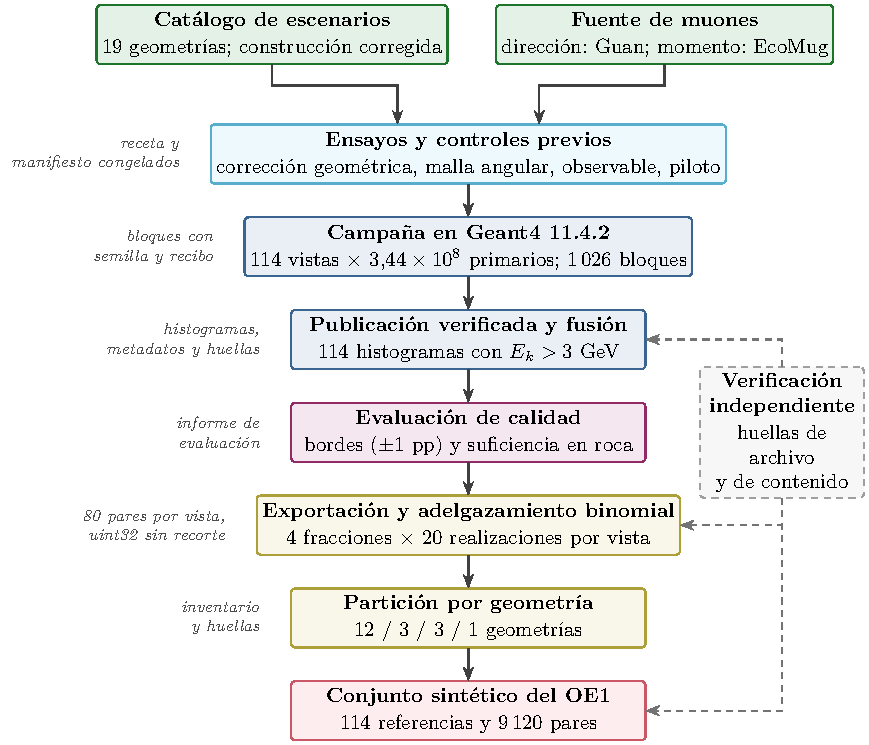
\includegraphics{fig3-1_flujo_oe1.pdf}
\caption[Cadena de generación y verificación del conjunto de datos (OE1)]{Cadena de generación y verificación del conjunto de datos sintéticos del OE1: insumos, ensayos y controles que fijaron la receta, campaña de Geant4 por bloques, publicación verificada y fusión, evaluación de calidad, exportación y adelgazamiento binomial, y partición por geometría. Las anotaciones de la izquierda indican los productos que enlazan cada etapa con la siguiente; la verificación independiente comprueba las huellas de archivo y de contenido. Fuente: elaboración propia a partir del repositorio de referencia.}
\label{fig:flujo}
\end{figure}

El desarrollo y la evaluación del modelo continuaron esa cadena a partir del conjunto particionado, como resume la \cref{fig:flujo-oe2}. Los pares de entrenamiento y validación, junto con la implementación corregida, alimentaron el piloto, cuyos pesos sirvieron de punto de partida a los ajustes por continuación y al ensayo de borde; durante todas esas etapas, el contrato de datos mantuvo cerradas las particiones de prueba y de generalización. Los pesos elegidos se congelaron por su huella en el contrato de la evaluación final, que se ejecutó después de registrar la procedencia de las particiones reservadas. Sus métricas se recalcularon de forma independiente, la selección de los controles de contraste recibió una corrección numérica y, por último, las mismas métricas se calcularon para la entrada sin red con cuatro fracciones de conteo. Cada etapa conservó, con sus productos, las configuraciones, los registros y las huellas que la enlazan con la anterior.

\begin{figure}[htbp]
\centering
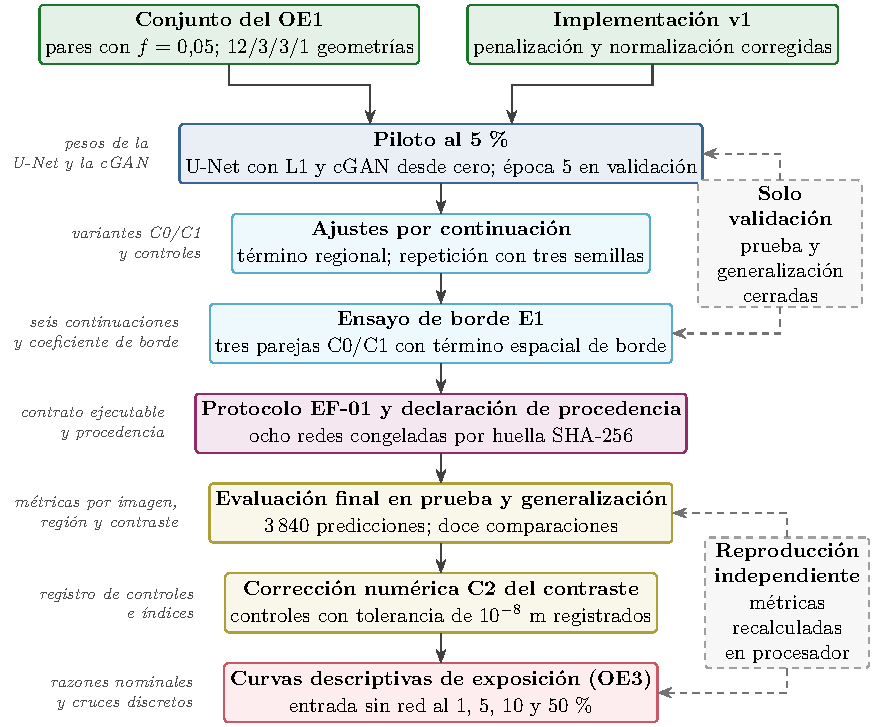
\includegraphics{fig3-6_flujo_oe2.pdf}
\caption[Desarrollo y evaluación del modelo (OE2) y análisis de exposición (OE3)]{Desarrollo y evaluación del modelo del OE2 y análisis descriptivo de exposición del OE3: insumos, ensayos decididos con validación, congelación de las redes y evaluación final, corrección numérica del contraste y curvas de exposición. Las anotaciones de la izquierda indican los productos que enlazan cada etapa con la siguiente; los recuadros discontinuos señalan la restricción de acceso a las particiones y la reproducción independiente de las métricas. Fuente: elaboración propia a partir del repositorio de referencia.}
\label{fig:flujo-oe2}
\end{figure}

% =============================================================================
\section{Generación y preparación del conjunto de datos sintéticos}
\label{sec:met-datos}

\subsection{Definición de los escenarios volcánicos y las anomalías}
\label{subsec:met-geometrias}

Cada escenario representó el edificio volcánico como un cono recto de radio basal $R$ y altura $H$, compuesto por roca homogénea de densidad 2,65~g\,cm$^{-3}$, en cuyo interior se insertaron anomalías de tres tipos: conductos de menor densidad, cavidades casi vacías y cuerpos más densos que la roca. Esta representación idealiza tres estructuras de interés en la exploración volcánica y mantiene, al mismo tiempo, espesores de roca de cientos de metros a algo más de un kilómetro a lo largo de las líneas de visión, el intervalo en el que la muografía por transmisión es factible con detectores de pocos metros cuadrados \parencite{lesparre2010,lechmann2021}. Las simplificaciones son deliberadas y explícitas: simetría cónica, roca de densidad única, anomalías de forma geométrica elemental con densidad uniforme y ausencia de topografía circundante. El alcance de la representatividad que se deriva de ellas se discute al final de esta sección.

El catálogo se generó de forma determinista. Cada geometría recibió una receta que fija su partición y su combinación de anomalías, y sus parámetros se muestrearon de distribuciones uniformes con un generador pseudoaleatorio independiente por geometría, derivado de una semilla común de valor 20260805 \parencite{harris2020}; así, el catálogo completo puede regenerarse exactamente. El diseño exigió que cada tipo de anomalía apareciera solo y en combinación con los demás, e incluyó una geometría de control sin anomalías y una geometría de generalización reservada fuera de toda partición de ajuste. La \cref{tab:rangos} presenta la parametrización del muestreo: el conducto es un cilindro vertical que parte de la base del edificio, la cavidad es una esfera y el cuerpo denso es un elipsoide de semiejes alineados con los ejes coordenados. En cavidades y cuerpos densos, el centro se desplazó del eje una fracción aleatoria del margen disponible, $\max\!\big(R(1-z_c/H)-r_h-20;\;30\big)$~m, donde $z_c$ es la altura del centro y $r_h$ el radio de la cavidad o el mayor semieje horizontal del cuerpo denso; el ángulo azimutal del centro fue uniforme en $[0;\,2\pi)$. Las longitudes se redondearon a 0,1~m y las densidades a tres decimales.

\begin{table}[htbp]
\centering
\caption[Parametrización del muestreo de los escenarios volcánicos]{Parametrización del muestreo de los escenarios volcánicos. $\mathcal{U}(a;\,b)$ denota una distribución uniforme en $[a;\,b]$; $H$ es la altura del edificio, $R$ su radio basal, $z_0$ y $z_1$ las alturas inferior y superior del conducto, $c_x$ y $c_y$ las coordenadas horizontales de su eje y $z_c$ la altura del centro de la anomalía. Fuente: elaboración propia a partir del generador del catálogo del repositorio de referencia.}
\label{tab:rangos}
\small
\begin{tabularx}{\linewidth}{@{}lX@{}}
\toprule
Elemento & Parámetros \\
\midrule
Edificio (cono) & $R\sim\mathcal{U}(500;\,700)$~m; $H\sim\mathcal{U}(350;\,450)$~m; densidad de la roca 2,65~g\,cm$^{-3}$ (fija) \\
Conducto (cilindro) & radio $\mathcal{U}(15;\,40)$~m; densidad $\mathcal{U}(1{,}8;\,2{,}2)$~g\,cm$^{-3}$; $c_x,c_y\sim\mathcal{U}(-40;\,40)$~m; $z_0=0$; $z_1=\mathcal{U}(0{,}75;\,0{,}95)\,H$ \\
Cavidad (esfera) & radio $\mathcal{U}(20;\,50)$~m; densidad $\mathcal{U}(0{,}0;\,0{,}5)$~g\,cm$^{-3}$; $z_c=\mathcal{U}(0{,}25;\,0{,}55)\,H$; desplazamiento radial $\mathcal{U}(0{,}1;\,0{,}6)$ del margen disponible \\
Cuerpo denso (elipsoide) & semiejes $a_x,a_y\sim\mathcal{U}(40;\,90)$~m, $a_z\sim\mathcal{U}(30;\,70)$~m; densidad $\mathcal{U}(3{,}0;\,3{,}3)$~g\,cm$^{-3}$; $z_c=\mathcal{U}(0{,}15;\,0{,}45)\,H$; desplazamiento radial $\mathcal{U}(0{,}1;\,0{,}5)$ del margen disponible \\
\bottomrule
\end{tabularx}
\end{table}

El resultado de ese muestreo es el catálogo de diecinueve escenarios que recoge la \cref{tab:catalogo}: doce destinados al entrenamiento, tres a la validación, tres a la prueba y uno a la evaluación de generalización. La tabla enumera, para cada geometría, las dimensiones del edificio y la densidad y el tamaño de cada anomalía en el orden en que se declararon, orden que resulta relevante cuando dos anomalías se superponen.

\begin{table}[htbp]
\centering
\caption[Catálogo de escenarios volcánicos sintéticos]{Catálogo de escenarios volcánicos sintéticos. C: conducto (densidad en g\,cm$^{-3}$; radio $r$ en m); V: cavidad (densidad; radio); D: cuerpo denso (densidad; semiejes $a_x/a_y/a_z$ en m). La densidad de la roca es 2,65~g\,cm$^{-3}$ en todos los casos; las anomalías se listan en el orden de declaración. Fuente: elaboración propia a partir del catálogo del repositorio de referencia.}
\label{tab:catalogo}
\footnotesize
\begin{tabularx}{\linewidth}{@{}llrrX@{}}
\toprule
Geometría & Partición & $R$ (m) & $H$ (m) & Anomalías \\
\midrule
geo-train-01 & entrenamiento & $656{,}2$ & $359{,}1$ & ninguna (control) \\
geo-train-02 & entrenamiento & $549{,}7$ & $409{,}8$ & C ($1{,}920$; $r=19{,}9$) \\
geo-train-03 & entrenamiento & $573{,}7$ & $356{,}2$ & V ($0{,}267$; $r=35{,}8$) \\
geo-train-04 & entrenamiento & $679{,}8$ & $387{,}2$ & D ($3{,}022$; $78{,}1/62{,}8/40{,}7$) \\
geo-train-05 & entrenamiento & $565{,}7$ & $386{,}0$ & C ($2{,}013$; $r=28{,}2$); V ($0{,}335$; $r=29{,}4$) \\
geo-train-06 & entrenamiento & $509{,}7$ & $416{,}3$ & C ($1{,}832$; $r=21{,}0$); D ($3{,}285$; $72{,}9/61{,}6/64{,}6$) \\
geo-train-07 & entrenamiento & $678{,}7$ & $429{,}2$ & V ($0{,}169$; $r=48{,}0$); D ($3{,}015$; $70{,}3/65{,}8/46{,}4$) \\
geo-train-08 & entrenamiento & $588{,}2$ & $413{,}4$ & C ($1{,}991$; $r=35{,}4$); V ($0{,}468$; $r=20{,}2$); D ($3{,}256$; $43{,}2/62{,}2/57{,}2$) \\
geo-train-09 & entrenamiento & $549{,}4$ & $373{,}2$ & C ($1{,}884$; $r=18{,}4$) \\
geo-train-10 & entrenamiento & $648{,}7$ & $449{,}6$ & V ($0{,}464$; $r=27{,}9$); V ($0{,}068$; $r=45{,}7$) \\
geo-train-11 & entrenamiento & $623{,}0$ & $419{,}8$ & C ($1{,}972$; $r=22{,}7$); V ($0{,}327$; $r=42{,}5$); V ($0{,}157$; $r=48{,}9$) \\
geo-train-12 & entrenamiento & $534{,}5$ & $411{,}9$ & D ($3{,}159$; $57{,}5/57{,}4/39{,}5$) \\
geo-val-01 & validación & $698{,}7$ & $427{,}6$ & C ($2{,}071$; $r=25{,}3$) \\
geo-val-02 & validación & $664{,}0$ & $367{,}3$ & V ($0{,}208$; $r=38{,}8$) \\
geo-val-03 & validación & $610{,}9$ & $425{,}4$ & C ($1{,}850$; $r=22{,}5$); D ($3{,}014$; $65{,}5/68{,}5/34{,}5$) \\
geo-test-01 & prueba & $671{,}1$ & $428{,}0$ & C ($2{,}151$; $r=30{,}3$); V ($0{,}454$; $r=36{,}5$) \\
geo-test-02 & prueba & $642{,}2$ & $415{,}9$ & D ($3{,}090$; $52{,}3/41{,}9/39{,}6$) \\
geo-test-03 & prueba & $518{,}5$ & $385{,}8$ & C ($1{,}914$; $r=30{,}2$); V ($0{,}222$; $r=24{,}1$); D ($3{,}244$; $74{,}2/55{,}3/64{,}9$) \\
geo-gen-01 & generalización & $619{,}2$ & $425{,}4$ & C ($1{,}831$; $r=26{,}1$); V ($0{,}242$; $r=40{,}9$); V ($0{,}048$; $r=42{,}4$) \\
\bottomrule
\end{tabularx}
\end{table}

La \cref{fig:catalogo} muestra un corte vertical de densidad de cada escenario, trazado por el plano que atraviesa la primera anomalía. Los cortes se calcularon con el campo de materiales del motor analítico que se describe en la sección~\ref{subsec:met-campana}, no con la construcción de Geant4, y permiten apreciar la variedad de tamaños, profundidades y combinaciones del catálogo.

\begin{figure}[htbp]
\centering
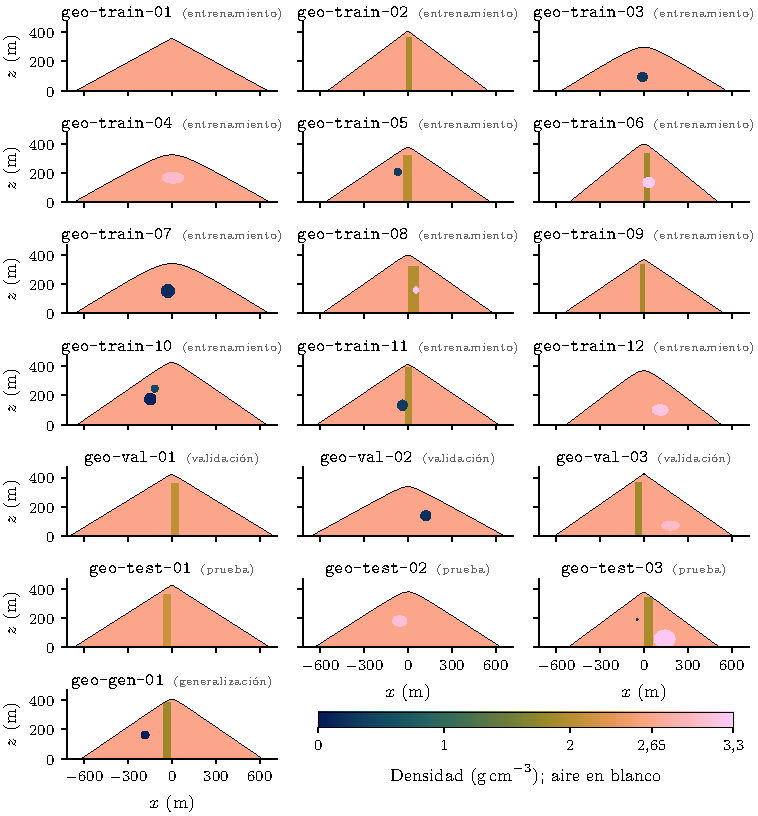
\includegraphics{fig3-2_catalogo_cortes.pdf}
\caption[Cortes verticales de densidad de los diecinueve escenarios]{Cortes verticales $x$--$z$ de densidad de los diecinueve escenarios del catálogo, por el plano $y$ que atraviesa la primera anomalía de cada geometría, calculados con el campo de materiales del motor analítico, a la misma escala horizontal y vertical. El aire se muestra en blanco. Fuente: elaboración propia a partir del catálogo del repositorio de referencia.}
\label{fig:catalogo}
\end{figure}

En la aplicación de transporte, basada en Geant4 \parencite{agostinelli2003,allison2016}, el edificio se construyó como un cono truncado con radio de vértice de 0,1~m, apoyado sobre el plano $z=0$ dentro de un volumen de aire. La roca se modeló como SiO$_2$ con la densidad del escenario, y cualquier densidad inferior a 0,05~g\,cm$^{-3}$ se sustituyó por aire, regla que en el catálogo afecta únicamente a la segunda cavidad de geo-gen-01. Cada anomalía se representó con su sólido elemental, del mismo material con su densidad propia, y se colocó como volumen hijo del edificio. En el conjunto inicial, las anomalías se colocaron completas, sin recortarlas al edificio ni restarlas entre sí, mientras que el motor analítico recorta cada anomalía al edificio y asigna a una región compartida la densidad de la última anomalía declarada; por esa diferencia, un mismo escenario no producía necesariamente el mismo campo de materiales en ambos motores cuando dos anomalías se superponían o una de ellas sobresalía del edificio. En la campaña definitiva, todas las geometrías se construyeron con la regla de corrección que se describe en la sección~\ref{subsec:met-verificacion}, la cual reproduce la convención del motor analítico.

La contención y el solapamiento de volúmenes se controlaron en dos niveles. Durante la construcción, Geant4 verificó cada colocación y emitió advertencias de superposición en el registro de la ejecución, sin detenerla. Sobre el catálogo se aplicó, además, una auditoría analítica independiente de la simulación. Para cada par de anomalías, la auditoría descartó la intersección solo mediante pruebas suficientes, como cajas envolventes disjuntas o distancias exactas entre esferas y cilindros; en los demás casos buscó puntos estrictamente interiores a ambos sólidos en una malla de $33\times33\times33$ puntos sobre la región común de sus cajas envolventes, y declaró el par intersectado solo al encontrar un testigo interior, dejando como no resuelta una búsqueda sin testigo. La contención de un conducto en el edificio se evaluó comparando su máximo radio ocupado, $\sqrt{c_x^2+c_y^2}+r$, con el radio del cono a la altura de su extremo superior, dado por la \cref{eq:radio-cono},
\begin{equation}
R(z)=R-(R-0{,}1)\,\frac{z}{H},
\label{eq:radio-cono}
\end{equation}
donde $R(z)$ es el radio del cono construido en Geant4 a la altura $z$, en metros, y 0,1~m su radio de vértice; para esferas y elipsoides se emplearon cotas suficientes y sus extremos verticales. Ninguno de los dos controles reproduce la navegación de las partículas, de modo que la ausencia de defectos en ellos no certifica por sí sola la geometría efectivamente transportada. Las superposiciones detectadas en el conjunto inicial motivaron la corrección y los ensayos descritos en la sección~\ref{subsec:met-verificacion}.

\paragraph{Representatividad dentro del alcance adoptado.}
% PENDIENTE (valoración de la dirección, criterio A-02): este apartado integra el
% borrador de representatividad de la rama de entrega (REPRESENTATIVIDAD_A02.md).
Bajo el alcance idealizado que adoptó la dirección, la representatividad del conjunto se entendió como la cobertura de una familia de edificios cónicos con heterogeneidades internas del tipo que la muografía volcánica asocia con conductos, cavidades y cuerpos densos \parencite{tanaka2007asama,olah2018sakurajima,tanaka2023muography}, observados en geometría de transmisión. No se pretendió que las geometrías reprodujeran un volcán concreto ni que las imágenes equivalieran a las de un instrumento real. Dentro de esa familia, el catálogo cubre edificios de 509,7 a 698,7~m de radio basal y de 356,2 a 449,6~m de altura; once conductos, en once geometrías, con densidades de 1,831 a 2,151~g\,cm$^{-3}$ y radios de 18,4 a 35,4~m; trece cavidades, en diez geometrías, con densidades de 0,048 a 0,468~g\,cm$^{-3}$ y radios de 20,2 a 48,9~m, y ocho cuerpos densos, en ocho geometrías, con densidades de 3,014 a 3,285~g\,cm$^{-3}$ y semiejes de 34,5 a 78,1~m. Las anomalías presentan contrastes de ambos signos respecto de la roca y aparecen solas y combinadas, incluidas dos geometrías con los tres tipos. La geometría de generalización repite la combinación de geo-train-11, con otros tamaños y posiciones, de modo que evalúa la generalización a nuevas configuraciones de anomalías conocidas y no a un tipo nuevo de anomalía.

En el cono homogéneo de cada geometría, el percentil 90 del espesor másico nominal de los rayos que cruzan roca va de $2{,}13\times10^{5}$ a $2{,}96\times10^{5}$~g\,cm$^{-2}$, y entre el 70,7 y el 87,1\,\% de las celdas de $4\times4$ píxeles con roca superan $10^{5}$~g\,cm$^{-2}$; las imágenes abarcan, por tanto, desde el cielo abierto hasta opacidades altas. El plan de trabajo preveía perfiles inspirados en topografías reales, como las de los volcanes Asama o Sakurajima, adaptados a geometrías simplificadas; el catálogo empleó conos, y esa simplificación se declara como una limitación del conjunto. La fuente y el transporte, descritos en las dos subsecciones siguientes, son únicos y trazables para las 114 vistas, y la tarea de los objetivos posteriores depende de la relación entre conteos de distinta estadística bajo esa definición común, no de una escala absoluta de flujo. Esa justificación respalda la representatividad dentro de la familia idealizada; no respalda la reproducción de un volcán concreto, un flujo calibrado ni la equivalencia con un detector. La valoración académica de este criterio corresponde a la dirección del proyecto.

\subsection{Configuración de la fuente de muones}
\label{subsec:met-fuente}

La fuente de muones debía cumplir dos requisitos: reproducir la distribución direccional del flujo con la misma convención que el motor analítico, para que ambas simulaciones fueran comparables, y conservar la física de un generador de muones cósmicos establecido. Para satisfacerlos se combinaron dos modelos. La dependencia direccional y la normalización se tomaron de la parametrización del flujo a nivel del mar de \textcite{guan2015muonflux}, que modifica la fórmula de Gaisser \parencite{gaisser2016} para energías bajas y ángulos cenitales grandes. El espectro de momento y la razón de carga se tomaron del generador EcoMug \parencite{pagano2021}.

EcoMug se empleó en una generación directa, independiente de Geant4, que produjo una muestra de $10^7$ muones desde un plano horizontal de cielo, con momento entre 0,5 y 10\,000~GeV/$c$ y semilla 20260805. A partir de esa muestra y de la parametrización de Guan se construyeron tres tablas que la aplicación de transporte consulta durante la simulación, sin invocar EcoMug en tiempo de ejecución. La primera asigna a cada una de las 256 filas angulares de elevación un peso proporcional al número esperado de muones de cielo abierto; la segunda almacena, para 16 bandas de elevación entre 2° y 47°, los cuantiles de la distribución del momento; y la tercera registra la razón de carga medida en la muestra. En la campaña definitiva, la generación se extendió 5° fuera de la ventana de observación, con el fin de compensar la migración angular de los muones desde el exterior de la ventana: el acimut se generó de manera uniforme en $\pm35^{\circ}$, los pesos de las ocho filas más próximas a cada borde de elevación se extrapolaron linealmente fuera del intervalo tabulado, con los pesos negativos anulados, y fuera del intervalo de las bandas de momento se empleó la banda extrema más cercana. La \cref{tab:generador} resume esa configuración.

\begin{table}[htbp]
\centering
\caption[Configuración de la fuente de muones]{Configuración de la fuente de muones de la campaña definitiva: muestra de EcoMug, tablas derivadas y extensión de la generación. Fuente: elaboración propia a partir de la receta operativa y de las tablas del generador del repositorio de referencia.}
\label{tab:generador}
\small
\begin{tabularx}{\linewidth}{@{}>{\raggedright\arraybackslash}p{5.0cm}>{\raggedright\arraybackslash}X@{}}
\toprule
Elemento & Valor registrado \\
\midrule
Versión de EcoMug & 2.2 (cabecera incluida en el código) \\
Muestra de EcoMug & $10^7$ muones; momento 0,5--10\,000~GeV/$c$; semilla 20260805 \\
Pesos por fila de elevación & 256 filas entre 2° y 47°, proporcionales al conteo de cielo abierto; ocho filas de borde extrapoladas linealmente fuera del intervalo \\
Distribución del momento & 16 bandas de elevación entre 2° y 47°; 257 cuantiles por banda; interpolación lineal; banda extrema fuera del intervalo \\
Razón de carga $\rho_{\pm}=\mu^+/\mu^-$ & 1,2794 \\
Ventana de generación & acimut relativo $\pm35^{\circ}$ (margen de 5° sobre la ventana de conteo) \\
Probabilidad de dirección nominal en la ventana, $p_{\mathrm{nom}}$ & 0,6841465610 \\
Escala convencional, $S_0$ & $36\,034\,069{,}91$ muones por 30 días convencionales \\
\bottomrule
\end{tabularx}
\end{table}

Las magnitudes que definen el muestreo y su normalización se agrupan en la \cref{eq:fuente}. El conteo esperado de cielo abierto en el píxel $(i,j)$, de la fila de elevación $i$ y la columna de acimut $j$, sigue la convención de aceptancia del protocolo de simulación (\cref{eq:fuente-lambda}); su suma sobre las columnas da el peso de cada fila, $\lambda_i$, y la suma de los pesos de todas las filas da la escala $S_0$ (\cref{eq:fuente-s0}). La fila de una dirección se elige con la probabilidad $w_i$ de la \cref{eq:fuente-w}, la carga positiva con la probabilidad de la \cref{eq:fuente-carga}, y la exposición convencional de una vista se obtiene de su número de direcciones nominales en la ventana según la \cref{eq:fuente-t}:
\begin{subequations}\label{eq:fuente}
\begin{align}
\lambda_{\mathrm{open},ij} &= \Phi_{\mathrm{int}}\,A\,\Delta\Omega_{ij}\,t, \qquad \lambda_i=\sum_{j=1}^{256}\lambda_{\mathrm{open},ij}, \label{eq:fuente-lambda}\\
S_0 &= \sum_{i=1}^{256}\lambda_i, \label{eq:fuente-s0}\\
w_i &= \frac{\lambda_i}{S_0}, \label{eq:fuente-w}\\
P(\mu^+) &= \frac{\rho_{\pm}}{1+\rho_{\pm}}, \label{eq:fuente-carga}\\
T_v &= 30\,\frac{N_{\mathrm{nom},v}}{S_0}. \label{eq:fuente-t}
\end{align}
\end{subequations}
En estas expresiones, $\Phi_{\mathrm{int}}$ es el flujo integral de muones de cielo abierto en la dirección del píxel, por encima de la energía mínima de 0,798~GeV, que en la convención heredada corresponde al frenado continuo en 367,5~g\,cm$^{-2}$ de aire, en cm$^{-2}$\,s$^{-1}$\,sr$^{-1}$; $A=1{,}44\times10^{4}$~cm$^{2}$ es el área de detección, tomada normal a cada dirección; $\Delta\Omega_{ij}=\Delta\alpha\,\Delta e\,\cos e_i$ es el ángulo sólido del píxel, en sr; $t$ es la duración de 30 días expresada en segundos; $\rho_{\pm}$ es la razón de carga de la \cref{tab:generador}; $N_{\mathrm{nom},v}$ es el número de primarios de la vista $v$ cuya dirección nominal cae dentro de la ventana de conteo, que se registró exactamente en cada bloque, y $T_v$ es la exposición convencional de la vista, en días convencionales. A diferencia del conjunto inicial, en el que el número de eventos de una simulación se sorteaba según una distribución de Poisson de media proporcional a la exposición, en la campaña definitiva cada vista recibió un número fijo de primarios, $N_v=3{,}44\times10^{8}$, de los cuales aproximadamente la fracción $p_{\mathrm{nom}}$ tiene dirección nominal en la ventana. La exposición $T_v$ es, por tanto, una etiqueta derivada de los supuestos del modelo de flujo y del área de detección, y no la duración de una medición de un detector real.

El algoritmo~\ref{alg:primario} describe cómo se generó cada muon a partir de esas tablas. La elevación se obtiene de la fila elegida más una perturbación uniforme de medio paso, el acimut es uniforme en la ventana de generación y el momento se obtiene invirtiendo la distribución acumulada de la banda correspondiente. La energía cinética se calcula como $E_k=\sqrt{p^2+m_\mu^2}-m_\mu$, en GeV, con $m_\mu=0{,}1056583745$~GeV/$c^2$ y $c=1$. El punto de inyección se sitúa sobre la trayectoria nominal que termina en el panel detector, según se explica en la sección~\ref{subsec:met-transporte}. Esta combinación reproduce la aceptancia direccional del motor analítico, de modo que las diferencias entre ambos motores reflejan la física del transporte, mientras que el espectro conserva la física del generador. El espectro de EcoMug es más blando que el de Guan, con distancias de Kolmogórov--Smirnov entre 0,063 y 0,119 según la banda de elevación; esa diferencia, junto con la masa de probabilidad que procede de las filas extrapoladas, forma parte de las hipótesis comunes del conjunto y no de un flujo calibrado.

\begin{algorithm}[htbp]
\caption{Generación dirigida de un muon primario a partir de las tablas del generador}
\label{alg:primario}
\begin{algorithmic}[1]
\Require pesos de fila $\{w_i\}$, incluidas las filas extrapoladas; cuantiles de momento por banda de elevación; razón de carga $\rho_{\pm}$; posición y orientación del panel detector; geometría del edificio; generador pseudoaleatorio inicializado con la semilla del bloque
\Ensure dirección, momento, carga y punto de inyección de un muon primario
\State elegir la fila de elevación $i$ con probabilidad $w_i$ mediante la distribución acumulada de los pesos
\State $e \gets$ centro de la fila $i$ más una perturbación uniforme en $\pm$ medio paso de fila
\State $\alpha \gets$ acimut relativo uniforme en $[-35^{\circ};\,35^{\circ}]$
\State $p \gets$ inversión de la distribución acumulada del momento en la banda de $e$, con interpolación lineal entre cuantiles
\State asignar carga positiva con probabilidad $\rho_{\pm}/(1+\rho_{\pm})$ y carga negativa en otro caso
\State $E_k \gets \sqrt{p^2+m_\mu^2}-m_\mu$
\State $\mathbf{x}_{\mathrm{imp}} \gets$ punto uniforme sobre la superficie del panel detector
\State muestrear la recta que parte de $\mathbf{x}_{\mathrm{imp}}$ hacia el cielo en la dirección $(e,\alpha)$ cada 0,5~m, hasta 4~km
\If{algún punto muestreado cae dentro del cono}
  \State $\mathbf{x}_0 \gets$ último punto interior encontrado, desplazado 1~m hacia el cielo
\Else
  \State $\mathbf{x}_0 \gets$ punto situado 1~m antes del panel sobre la misma recta
\EndIf
\State \Return $(\mathbf{x}_0,\ e,\ \alpha,\ E_k,\ \text{carga})$
\end{algorithmic}
\end{algorithm}

\subsection{Transporte de partículas y representación del detector en Geant4}
\label{subsec:met-transporte}

El transporte se simuló con una aplicación desarrollada sobre Geant4 11.4.2, con la lista de física \texttt{FTFP\_BERT}. Como la variable de interés es el número de muones primarios que atraviesan el edificio, toda partícula secundaria se eliminó en el momento de su creación y solo se transportó el muon primario. Esta decisión reduce el costo computacional sin alterar la transmisión de primarios, aunque excluye del modelo los fondos producidos por secundarios. La ejecución se hizo en modo multihilo, con 64 hilos por bloque, y la semilla de cada bloque inicializó el generador de Geant4. La \cref{tab:geant4} resume la configuración del transporte y del registro.

\begin{table}[htbp]
\centering
\caption[Configuración del transporte y del registro en Geant4]{Configuración del transporte y del registro en Geant4 en la campaña definitiva. Fuente: elaboración propia a partir de la receta operativa y de los metadatos de la campaña del repositorio de referencia.}
\label{tab:geant4}
\small
\begin{tabularx}{\linewidth}{@{}lX@{}}
\toprule
Elemento & Configuración \\
\midrule
Geant4 & versión 11.4.2, modo multihilo; 64 hilos por bloque \\
Física & \texttt{FTFP\_BERT}; solo primarios, secundarios eliminados al crearse \\
Edificio y anomalías & cono de radio de vértice 0,1~m; roca SiO$_2$ a la densidad del escenario; anomalías construidas con la regla de corrección B1 \\
Panel detector nominal & $1{,}2\times1{,}2$~m; a 1\,000~m del eje y 1,5~m de altura; vista $v$ en el acimut $60^{\circ}\,v$ \\
Punto de inyección & 1~m antes de la entrada en la roca sobre la trayectoria nominal (algoritmo~\ref{alg:primario}) \\
Plano de conteo & cuadrado de $600\times600$~m centrado en el panel \\
Registro & energía cinética al cruzar el plano de conteo superior a 3~GeV \\
Malla angular & $256\times256$; acimut relativo en 256 intervalos iguales de 0,234375° entre $-30^{\circ}$ y $30^{\circ}$; elevación en 256 centros entre 2° y 47° \\
Primarios por vista & $3{,}44\times10^{8}$, en nueve bloques \\
\bottomrule
\end{tabularx}
\end{table}

La simulación distinguió entre el detector físico y la superficie en la que se registran los muones, una distinción que la \cref{fig:geometria-observacion} ilustra. El panel detector nominal es un cuadrado de 1,2~m de lado, situado a 1\,000~m del eje del cono y a 1,5~m de altura, orientado hacia el eje; la vista $v$ lo ubica en el acimut $60^{\circ}\,v$. Para no desperdiciar tiempo de cómputo en muones que nunca alcanzarían el detector, el muestreo se dirigió: cada muon se generó sobre una trayectoria nominal que termina en un punto uniforme del panel. En el conjunto inicial, el punto de partida se situaba a una distancia fija más allá del borde lejano del edificio, de modo que el muon atravesaba cientos de metros de aire antes de llegar a la roca. Como el espectro tabulado corresponde al nivel del mar, ese recorrido descontaba dos veces la atenuación en el aire; por ello, en la campaña definitiva el muon se inyectó 1~m antes de su entrada en la roca, siguiendo el algoritmo~\ref{alg:primario}, y 1~m antes del panel cuando la trayectoria no cruza roca.

\begin{figure}[htbp]
\centering
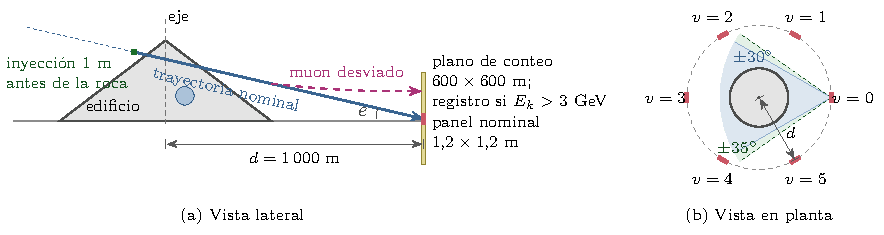
\includegraphics{fig3-3_geometria_observacion.pdf}
\caption[Geometría de observación de la simulación]{Geometría de observación de la campaña definitiva. (a)~Vista lateral: edificio cónico, panel detector nominal de $1{,}2\times1{,}2$~m a la distancia $d$ del eje, plano de conteo de $600\times600$~m centrado en el panel, trayectoria nominal con el punto de inyección situado 1~m antes de la entrada en la roca y trayectoria de un muon desviado por dispersión múltiple. (b)~Vista en planta: seis posiciones del detector, separadas 60°, ventana de conteo de $\pm30^{\circ}$ y ventana de generación de $\pm35^{\circ}$ de la vista~0. Esquema sin escala. Fuente: elaboración propia a partir de la receta operativa.}
\label{fig:geometria-observacion}
\end{figure}

El registro, en cambio, se hizo sobre un plano de conteo mucho mayor que el panel: un cuadrado de $600\times600$~m centrado en él. Cuando el muon primario alcanza ese plano con energía cinética superior a 3~GeV, se calculan la elevación y el acimut de su dirección de llegada y se le asigna el píxel correspondiente de la malla angular. La razón de esta separación es la dispersión coulombiana múltiple \parencite{lynch1991}: a lo largo de cientos de metros de roca y de aire, los muones de pocos GeV se desvían decenas de metros de su trayectoria nominal, de modo que una superficie de registro del tamaño del panel perdería una fracción de los muones generados sobre él que depende de su energía. El umbral de 3~GeV elimina, además, los muones blandos dispersados cuya contribución dependía del tamaño del plano. Debe subrayarse que la independencia del conteo respecto del tamaño del plano, que se comprobó en los ensayos de la sección~\ref{subsec:met-verificacion}, es una convergencia del muestreo para una fuente restringida al panel nominal: no demuestra que la imagen sea la de un detector físico de 1,2~m expuesto a una fuente espacialmente amplia.

La malla angular sustituyó a la convención histórica del conjunto inicial, que asignaba cada dirección al más cercano de 256 centros equiespaciados entre $-30^{\circ}$ y $30^{\circ}$, de modo que los dos intervalos extremos tenían la mitad del ancho de los interiores. En la convención adoptada, el acimut relativo se divide en 256 intervalos iguales delimitados por bordes explícitos, mientras que en elevación se conservaron los 256 centros entre 2° y 47° de la convención histórica. Cada histograma se registró en tres versiones complementarias: con el umbral de 3~GeV, que constituye la referencia; sin umbral, y por dirección nominal de generación, esta última usada para contar exactamente $N_{\mathrm{nom},v}$. Ningún evento recibió un peso estadístico: todos tuvieron peso unitario, la dependencia direccional quedó contenida en el muestreo de filas y la exposición convencional en la \cref{eq:fuente-t}.

\subsection{Verificación de la cadena de simulación}
\label{subsec:met-verificacion}

La verificación se organizó siguiendo los eslabones de la cadena: el generador de muones, las geometrías y su corrección, la malla angular, el observable y su normalización, el piloto con la receta de producción y, finalmente, la calidad de las referencias de la campaña. La \cref{tab:verificacion} resume cada comprobación con su procedimiento, su criterio y su estado. Dos precisiones delimitan su alcance. La primera es que la bitácora del conjunto inicial se reconstruyó después de su campaña a partir de registros primarios, de modo que los procedimientos anteriores a la revisión técnica se describen con esa trazabilidad retrospectiva. La segunda es que varias comprobaciones se diseñaron y ejecutaron sobre el motor analítico, y su validez no se transfiere automáticamente al transporte con Geant4. Los resultados de todas ellas se presentan en el capítulo~\ref{chap:resultados}.

\begin{table}[htbp]
\centering
\caption[Comprobaciones de la cadena de simulación]{Comprobaciones de la cadena de simulación: procedimiento, criterio y estado. Los resultados se presentan en el capítulo~\ref{chap:resultados}. Fuente: elaboración propia a partir del repositorio de referencia.}
\label{tab:verificacion}
\small
\begin{tabularx}{\linewidth}{@{}>{\raggedright\arraybackslash}p{2.6cm}>{\raggedright\arraybackslash}X>{\raggedright\arraybackslash}p{3.4cm}>{\raggedright\arraybackslash}p{1.8cm}@{}}
\toprule
Eslabón & Procedimiento & Criterio & Estado \\
\midrule
Generador & muestreador y tablas frente a la parametrización de Guan & residuo relativo máximo $<10\,\%$; reproducción de $S_0$ & ejecutado \\
Generador & muestra de EcoMug frente a la parametrización de Guan & sin criterio; diferencia declarada como hipótesis & ejecutado \\
Geometrías & auditoría analítica y control geométrico de la regla B1 & \cref{tab:control-t} & ejecutado \\
Corrección & piloto A/B en geo-train-06 & partición de la \cref{eq:piloto} & ejecutado \\
Corrección & segundo ensayo con primarios compartidos y complemento dirigido & protocolo de la dirección; resultado inconcluso admitido & ejecutado \\
Malla angular & integración en el supercomputador con 1\,000 primarios & metadatos, histograma, registro y código de salida & ejecutado \\
Observable & planos de conteo, aire previo, bordes y asíntota & fijados antes de ejecutar & ejecutado \\
Observable & equivalencia con un panel físico & intervalo simultáneo en $[0{,}95;\,1{,}05]$ & no ejecutado \\
Piloto & seis vistas de geo-train-06 con la receta de producción & bordes con $\alpha=0{,}05/6$ & ejecutado \\
Campaña & integridad, bordes y suficiencia en roca & \cref{eq:bordes} y~\cref{eq:roca} & ejecutado \\
Reproducción & evaluación desde los píxeles y regeneración de pares & huellas de archivo y de contenido & ejecutado \\
\bottomrule
\end{tabularx}
\end{table}

\paragraph{Generador de muones.}
El muestreador del motor analítico se contrastó con la parametrización de \textcite{guan2015muonflux} mediante una muestra de $10^7$ muones. Se compararon el espectro de energía, en 40 intervalos logarítmicos entre 0,5 y 100~GeV, y la distribución del ángulo cenital $\zeta$, en 35 intervalos de $\cos\zeta$ entre 0° y 70°, y la validación se consideró superada solo si el residuo relativo máximo fue inferior al 10\,\% en ambas distribuciones. La muestra de EcoMug se comparó con la misma parametrización incorporando el factor de aceptancia $\cos\zeta$, necesario porque EcoMug genera el flujo que atraviesa una superficie horizontal; esta segunda comparación no tuvo un criterio de aprobación, porque EcoMug implementa su propia parametrización y una diferencia moderada entre modelos es esperable. Para la receta definitiva se recalculó, además, la escala $S_0$ directamente desde la parametrización de Guan y se comprobó, con una prueba de bondad de ajuste $\chi^2$ de 255 grados de libertad, que el generador reproducía la distribución de las direcciones por filas de elevación.

\paragraph{Transporte y normalización de cielo abierto en el motor analítico.}
Sobre el motor analítico se aplicaron cuatro pruebas físicas: la transmisión a través del edificio homogéneo frente a un cálculo teórico independiente, con error relativo máximo inferior a 0,15; la sensibilidad al contraste de una cavidad conocida de 40~m de radio y densidad nula, cuyo espesor másico y transmisión debían coincidir con los teóricos con el mismo error; la dispersión de Poisson de los conteos sobre 400 réplicas, con índice de dispersión medio a menos de 0,05 de la unidad y menos del 10\,\% de los píxeles fuera de la banda bilateral del 95\,\%; y la exactitud de la tabla de interpolación del flujo frente a la integración directa, con error relativo inferior a 0,01.

\paragraph{Corrección de la geometría geo-train-06.}
La auditoría del catálogo mostró que en seis escenarios las anomalías se superponían entre sí o sobresalían del edificio, y que Geant4 había emitido las advertencias correspondientes durante la campaña del conjunto inicial. Como en una región compartida por dos volúmenes hermanos Geant4 no define qué material se atraviesa, se diseñó una corrección y se ensayó primero en geo-train-06, donde un conducto y un cuerpo denso se intersectan. El diagnóstico previo estimó la intersección con $4\times10^6$ muestras uniformes en la caja envolvente común de ambas anomalías y verificó la contención del cuerpo denso sobre una parametrización de su superficie con paso angular de 0,25°. La corrección adoptada, denominada B1, define la región material que corresponde a cada anomalía mediante la \cref{eq:b1},
\begin{equation}
\mathcal{R}_i=\left(A_i\cap\mathcal{K}\right)\setminus\bigcup_{j>i}A_j ,
\label{eq:b1}
\end{equation}
donde $A_i$ es el sólido de la anomalía de índice $i$ en el orden de declaración, $\mathcal{K}$ es el cono del edificio y $\mathcal{R}_i$ es la región que recibe finalmente la densidad de la anomalía $i$. Cada anomalía se recorta al edificio y cede a las anomalías declaradas después la región que comparte con ellas. La regla coincide con la que ya aplicaba el motor analítico, de modo que ambos motores pasan a representar el mismo campo de materiales, y no modifica ningún parámetro publicado del catálogo. El algoritmo~\ref{alg:b1} muestra su implementación con sólidos booleanos de Geant4. El recorte al edificio se realizó contra un cono auxiliar interior al edificio por un margen de 1~mm, para evitar superficies coincidentes con el volumen madre; por ese margen, la correspondencia con el campo analítico no es exacta en las fronteras. Se consideraron y descartaron dos alternativas: dar prioridad al conducto, que introducía una divergencia nueva con el motor analítico, y desplazar el cuerpo denso, que alteraba el escenario físico publicado.

\begin{algorithm}[htbp]
\caption{Construcción de los volúmenes de las anomalías con la regla B1}
\label{alg:b1}
\begin{algorithmic}[1]
\Require sólidos de las anomalías $A_1,\dots,A_m$ en el orden de declaración; cono del edificio $\mathcal{K}$; cono auxiliar $\mathcal{K}^{-}$, interior a $\mathcal{K}$ por 1~mm
\Ensure volúmenes colocados que realizan las regiones $\mathcal{R}_1,\dots,\mathcal{R}_m$ de la \cref{eq:b1}
\For{$i \gets 1$ \textbf{hasta} $m$}
  \State $S \gets A_i$
  \If{una prueba suficiente no certifica que $A_i$ está contenida en $\mathcal{K}$}
    \State $S \gets S \cap \mathcal{K}^{-}$ \Comment{intersección booleana}
  \EndIf
  \For{$j \gets i+1$ \textbf{hasta} $m$}
    \If{las cajas envolventes de $A_i$ y $A_j$ se superponen}
      \State $S \gets S \setminus A_j$ \Comment{sustracción booleana}
    \EndIf
  \EndFor
  \If{$S$ no es vacío}
    \State colocar $S$ como volumen hijo de $\mathcal{K}$ con la densidad de la anomalía $i$
  \Else
    \State registrar en el diagnóstico que la anomalía $i$ no se coloca
  \EndIf
\EndFor
\end{algorithmic}
\end{algorithm}

La corrección se evaluó comparando dos ejecutables compilados desde la misma base de código: la variante~A, que conserva la geometría original como referencia de diagnóstico, y la variante~B, que incorpora la regla B1. Primero se ejecutó un control geométrico en cuatro tareas, cuyo diseño y criterios resume la \cref{tab:control-t}. La primera tarea buscó superposiciones en las 19 geometrías, las 6 vistas y ambas variantes; las siguientes contrastaron la construcción de geo-train-06 con el motor analítico mediante sondeos puntuales, volúmenes y cortes, y la última comprobó que una simulación ordinaria de la variante~B terminara sin advertencias geométricas. Los volúmenes de las cuatro intersecciones del catálogo se contrastaron, además, en la revisión de la dirección, mediante una integración numérica independiente por cuadratura adaptativa. Ninguno de estos controles mide el efecto de la corrección sobre los conteos, que es el objeto de los ensayos siguientes.

\begin{table}[htbp]
\centering
\caption[Diseño del control geométrico de la corrección B1]{Diseño del control geométrico de la corrección B1. A: variante con la geometría original; B: variante con la regla B1 (\cref{eq:b1}). Fuente: elaboración propia a partir de la entrega del ensayo de corrección.}
\label{tab:control-t}
\small
\begin{tabularx}{\linewidth}{@{}lXX@{}}
\toprule
Tarea & Procedimiento & Criterio \\
\midrule
T1 & búsqueda de superposiciones con $10^5$ puntos por volumen y tolerancia nula en 19 geometrías, 6 vistas y 2 variantes (228 ejecuciones) & B sin superposiciones; A con superposiciones solo en las geometrías señaladas por la auditoría \\
T2 & en geo-train-06, vista~0: sondeos puntuales del navegador, volúmenes de las anomalías con $10^7$ muestras y dos cortes frente al motor analítico & sondeos coincidentes; volúmenes dentro de tres errores estándar combinados; discrepancias de corte explicadas como borde o como clase aire \\
T3 & mapas de material y de discrepancia en los dos cortes & inspección visual \\
T4 & simulación ordinaria de geo-train-06, vista~0, con $10^4$ eventos & B completa, sin advertencias geométricas, con histograma no vacío y totales coherentes; A como referencia \\
\bottomrule
\end{tabularx}
\end{table}

\paragraph{Ensayo piloto de la corrección.}
El ensayo piloto comparó las variantes A y B sobre la vista~0 de geo-train-06, con $10^6$ eventos por simulación, tres semillas y las mismas tablas, física y recursos en ambas variantes. Antes de enviar las simulaciones se registraron en un prerregistro cinco regiones de interés derivadas exclusivamente de la geometría, por trazado de rayos sobre la rejilla angular y nunca a partir de las imágenes medidas: la intersección entre las anomalías, el conducto exclusivo, el cuerpo denso exclusivo, la roca sin anomalías y el cielo, estas dos últimas como controles. El mismo prerregistro acotó el efecto máximo esperado, $\Delta_{\max}$, como la diferencia de conteos entre suponer que el cuerpo denso ocupa la intersección y suponer que la ocupa el conducto, y anticipó que, con ese número de eventos, la región de intersección no tendría potencia suficiente para distinguir las variantes. Para cada región y semilla $s$ se definieron la diferencia emparejada, su media y su error estándar, y los resultados posibles se particionaron de antemano en cuatro casos según la \cref{eq:piloto}:
\begin{subequations}\label{eq:piloto}
\begin{align}
d_s &= C_{B,s}-C_{A,s}, \qquad \bar d=\frac{1}{3}\sum_{s=1}^{3}d_s, \qquad \mathrm{EE}=\frac{\mathrm{SD}(d_s)}{\sqrt{3}}, \label{eq:piloto-dif}\\
\mathrm{EE}_{\mathrm{prev}} &= \sqrt{2N_{\mathrm{B1}}/3}, \label{eq:piloto-ee}\\
\text{resultado} &=
\begin{cases}
\text{inconcluso}, & \mathrm{EE}_{\mathrm{prev}}>|\Delta_{\max}|,\\
\text{nulo}, & |\bar d|\le 2\,\mathrm{EE}_{\mathrm{prev}},\\
\text{efecto presente}, & |\bar d|>2\,\mathrm{EE}_{\mathrm{prev}}\ \text{y compatible con}\ \Delta_{\max},\\
\text{discordante}, & |\bar d|>2\,\mathrm{EE}_{\mathrm{prev}}\ \text{e incompatible con}\ \Delta_{\max}.
\end{cases} \label{eq:piloto-decision}
\end{align}
\end{subequations}
En estas expresiones, $C_{V,s}$ es el conteo total dentro de la región para la variante $V$ y la semilla $s$; $\mathrm{SD}(d_s)$ es la desviación estándar de las tres diferencias; $\mathrm{EE}$ es el error estándar observado, y $\mathrm{EE}_{\mathrm{prev}}$ es el error estándar previsto a partir del conteo esperado por simulación bajo la regla B1, $N_{\mathrm{B1}}$. Los tres últimos casos de la \cref{eq:piloto-decision} solo se aplican cuando $\mathrm{EE}_{\mathrm{prev}}\le|\Delta_{\max}|$: un resultado inconcluso indica que la estadística planeada no tenía, de partida, capacidad para separar el valor nulo de $\Delta_{\max}$, y no debe interpretarse como evidencia de que las variantes sean equivalentes; un resultado nulo, en cambio, se obtiene con potencia adecuada; una diferencia es compatible con $\Delta_{\max}$ cuando tiene su mismo signo y no lo supera ampliamente en magnitud; y un resultado discordante exige investigar el procedimiento antes de cualquier conclusión. El umbral de dos errores estándar es una regla heurística y no un intervalo de Student, pues con tres semillas el valor crítico exacto sería $t_{0{,}975;\,2}\approx4{,}303$. Las regiones de control debían mostrar diferencias compatibles con cero, lo que permite descartar diferencias espurias del procedimiento.

\paragraph{Segundo ensayo con correspondencia de primarios.}
Usar semillas iguales no garantiza que las variantes transporten los mismos muones, porque cambiar la geometría altera la secuencia de números aleatorios. Por ello, la dirección del proyecto definió un segundo ensayo en el que ambas variantes leen una misma lista de muones primarios generada de antemano y registran, para cada primario, si fue detectado, en qué píxel y si atravesó la región original de la intersección. Su primera etapa comprendió las geometrías geo-train-06 y geo-train-01, esta última sin anomalías como control, en su vista~0, con tres réplicas de la comparación A/B y una repetición técnica A/A, en 13 simulaciones de $10^5$ primarios con trazabilidad individual. Un complemento dirigido, con doce trayectorias que atraviesan la región compartida y tres semillas por variante, comprobó a qué material asigna cada variante esa región. La segunda etapa, regida por un protocolo revisado, fijó de antemano un tamaño de $2{,}4\times10^{7}$ pares principales de primarios, con 55 simulaciones y $4{,}87\times10^{7}$ transportes en total incluidos los controles; un margen operativo ligado al ruido de conteo de la región de interés; un intervalo de confianza conservador de al menos 95\,\% construido con límites binomiales exactos, y la admisión explícita de un resultado inconcluso, sin ampliación automática del tamaño.

\paragraph{Malla angular.}
La revisión del registro angular cuantificó la discretización de la convención histórica y motivó la adopción de la malla de intervalos iguales de la \cref{tab:geant4}. Su integración en la aplicación de transporte se comprobó en el supercomputador con una simulación de 1\,000 primarios, revisando los metadatos, el histograma, el registro de ejecución y el código de salida, antes de cualquier producción con la nueva malla.

\paragraph{Diagnóstico del observable y de la normalización.}
Para fijar el observable de la campaña se ejecutaron en el supercomputador cuatro controles cortos sobre la vista~0 de la geometría homogénea geo-train-01, cada uno con su pregunta, su comparación y su criterio de resultado establecidos antes de la ejecución. Un único plano de 1\,200~m registró a la vez cuadrados anidados de 1,2, 100, 300 y 600~m de lado con los mismos muones, de modo que la razón entre planos es una fracción binomial anidada. El primer control comparó, para varios umbrales de energía cinética y tres puntos de inyección, la razón de conteos entre los planos de 100 y 600~m por bandas de espesor másico de roca, con el criterio de una razón de al menos 0,98 en todas las bandas; el segundo midió la eficiencia de cielo abierto para decidir si el muon debía atravesar el aire previo; el tercero midió la desviación de las filas y columnas de borde frente al interior para varios márgenes angulares de generación; y el cuarto comparó los planos de 600 y 1\,200~m para comprobar la asíntota. Un quinto control, que habría comparado la imagen del estimador con la de un panel físico expuesto a una fuente espacialmente amplia, quedó diseñado con un criterio de equivalencia por intervalos simultáneos, pero no se ejecutó: su costo era elevado y el alcance adoptado no exige equivalencia instrumental.

\paragraph{Piloto de seis vistas.}
Con la receta de producción fijada, se ejecutó un piloto sobre las seis vistas de geo-train-06, con $2{,}11\times10^{8}$ primarios por vista en seis bloques. El piloto aplicó el criterio de bordes que se describe a continuación, con un error familiar del 5\,\% repartido entre sus seis vistas, y registró los mismos indicadores descriptivos de roca. Se evaluó una sola vez, con el número de primarios fijado, y sus resultados sirvieron para dimensionar el presupuesto de la campaña; sus histogramas no se sumaron a las referencias finales.

\paragraph{Criterios de calidad de la campaña.}
Las referencias de la campaña se evaluaron con tres criterios registrados antes del envío. El primero, de integridad, exigió exactamente 114 referencias compatibles, con el número de primarios, las semillas, la receta, las geometrías y las tablas del manifiesto, conteos enteros sin saturación y procedencia verificable; un error técnico impedía aceptar la vista. El segundo evaluó la respuesta en los bordes de la ventana frente a una referencia ideal de la fuente sin transporte. Para cada vista se definieron quince regiones de borde, formadas por las cinco columnas extremas de cada lado y las cinco filas superiores, restringidas al cielo entre 30° y 42° de elevación en el caso de las columnas, y una región interior con las columnas 20 a 235 en la misma banda de cielo. La respuesta de cada región se contrastó con la de la región interior según la \cref{eq:bordes}:
\begin{subequations}\label{eq:bordes}
\begin{align}
\hat p_r &= \frac{C_r}{N_v}, \label{eq:bordes-p}\\
\varepsilon_r &= \frac{\hat p_r-p^{\mathrm{ideal}}_r}{p^{\mathrm{nom}}_r}, \label{eq:bordes-e}\\
\Delta_r &= \varepsilon_r-\varepsilon_{\mathrm{int}}, \qquad \text{equivalente si}\ \left[\Delta_r^{-};\,\Delta_r^{+}\right]\subset\left[-0{,}01;\,0{,}01\right], \label{eq:bordes-d}
\end{align}
\end{subequations}
donde $C_r$ es el conteo de la región $r$ en la referencia; $N_v$ es el número de primarios de la vista; $\hat p_r$ es la probabilidad estimada de que un primario sea registrado en la región; $p^{\mathrm{ideal}}_r$ es la probabilidad de que la fuente ideal, sin transporte, produzca un primario con dirección en la región y energía cinética superior al umbral; $p^{\mathrm{nom}}_r$ es la probabilidad de que la dirección nominal de un primario caiga en la región; $\varepsilon_r$ es la respuesta relativa de la región y $\varepsilon_{\mathrm{int}}$ la de la región interior; y $\left[\Delta_r^{-};\,\Delta_r^{+}\right]$ es el intervalo del contraste. La resta de $p^{\mathrm{ideal}}_r$ ajusta el cambio del espectro con la elevación, y la tolerancia de 0,01 equivale a $\pm1$ punto porcentual de probabilidad de registro por inyección nominal. Cada probabilidad se trató como una proporción binomial de $N_v$ historias independientes, con a lo sumo una llegada registrada por primario, y se acotó con intervalos de \textcite{clopper1934}; con una corrección de Bonferroni \parencite{dunn1961}, el error familiar de 0,05 se repartió entre las 114 vistas y, dentro de cada vista, entre sus dieciséis probabilidades, y los extremos del contraste se obtuvieron restando los extremos de los intervalos, una cota simultánea conservadora que no supone independencia entre regiones.

El tercer criterio describió la suficiencia del conteo en la roca. Se predefinieron, sin observar los conteos, regiones de interés de $4\times4$ píxeles cuyo espesor másico nominal en el cono homogéneo, calculado por marcha de rayos de 2~m con el procedimiento del motor analítico de la sección~\ref{subsec:met-campana}, quedara entre $3\times10^{4}$ y $10^{5}$~g\,cm$^{-2}$. Esas máscaras ignoran las anomalías, que sí se transportan, y son comunes a las seis vistas de cada geometría por la simetría circular del cono homogéneo; contienen entre 150 y 244 regiones por geometría. Para cada vista se calculó el indicador de la \cref{eq:roca},
\begin{equation}
F_v=\frac{1}{M_v}\sum_{m=1}^{M_v}\mathbf{1}\!\left[C_{v,m}\geq100\right],
\label{eq:roca}
\end{equation}
donde $M_v$ es el número de regiones de roca de la vista, $C_{v,m}$ es la suma de los conteos de la referencia en la región $m$ y $\mathbf{1}[\cdot]$ es la función indicadora. La meta descriptiva, $F_v\geq0{,}90$, se acompañó de la mediana y el percentil 10 de los conteos por región. Cien cuentas representan aproximadamente un 10\,\% de ruido relativo de conteo en la región agregada, sin incluir la incertidumbre del modelo; el indicador no constituye una precisión por píxel, un criterio para toda la roca ni una garantía sobre las tasas verdaderas. El acuerdo previo con la dirección estableció que una vista por debajo de la meta se conservaría y se reportaría, sin aumentar el número de primarios, descartar imágenes ni modificar la regla después de conocer los resultados.

\subsection{Ejecución de la campaña y formación de imágenes}
\label{subsec:met-campana}

La campaña de transporte simuló las 114 vistas del catálogo en el supercomputador de la universidad (sección~\ref{subsec:met-entorno}), con un número fijo de $3{,}44\times10^{8}$ primarios por vista, para un total de $3{,}9216\times10^{10}$. Cada vista se dividió en nueve bloques, ocho de 38\,222\,223 primarios y uno de 38\,222\,216, de modo que la campaña comprendió 1\,026 bloques definidos en un manifiesto congelado antes del envío. Para que cualquier bloque pudiera repetirse de forma independiente, su semilla se derivó de manera determinista mediante la \cref{eq:semilla-campana},
\begin{equation}
s(g,v,b)=20261002\cdot10^{6}+6\cdot10^{5}+g\cdot10^{4}+v\cdot10^{2}+b ,
\label{eq:semilla-campana}
\end{equation}
donde $s$ es la semilla del bloque, $g\in\{0,\dots,18\}$ la posición de la geometría en el orden alfabético del catálogo, $v\in\{0,\dots,5\}$ la vista y $b\in\{0,\dots,8\}$ el índice del bloque. Las semillas son nuevas respecto de las del piloto, y ninguna se repite.

La ejecución se automatizó con un procedimiento idempotente, descrito en el algoritmo~\ref{alg:campana}, que tolera interrupciones y repeticiones sin corromper los resultados. En cada pasada, el procedimiento compara el manifiesto con los bloques ya publicados, omite los bloques con un trabajo en curso o con un intento previo sin conciliar y envía los bloques pendientes al gestor de trabajos. Cada trabajo simula su bloque en un directorio temporal y, al terminar, el bloque se publica solo después de verificar la copia y la huella SHA-256 \parencite{nist2015} de sus archivos frente al recibo, de modo que un bloque incompleto o alterado nunca llega al directorio de publicación. Un trabajo fallido se concilia con los registros del gestor antes de cualquier reintento, y ningún registro se borra para forzar un envío. La receta, el manifiesto y las herramientas se verificaron por sus huellas al inicio de cada trabajo, y la copia de trabajo no se modificó durante la campaña.

\begin{algorithm}[htbp]
\caption{Ejecución idempotente de la campaña por bloques}
\label{alg:campana}
\begin{algorithmic}[1]
\Require manifiesto congelado de bloques $\{(g,v,b,s,N_b)\}$; receta y herramientas con sus huellas; directorios temporal y de publicación
\Ensure un bloque publicado y verificado por cada fila del manifiesto
\Function{Pasada}{}
  \State verificar las huellas del manifiesto, la receta y las herramientas
  \State $\mathcal{F} \gets$ filas del manifiesto sin bloque publicado, excluidas las que tienen un trabajo en curso o un intento previo sin conciliar
  \For{cada fila $(g,v,b,s,N_b)$ de $\mathcal{F}$, dentro del cupo disponible}
    \State enviar un trabajo \Call{Simular}{$g,v,b,s,N_b$}
  \EndFor
\EndFunction
\Function{Simular}{$g,v,b,s,N_b$}
  \State transportar $N_b$ primarios de la vista $v$ de la geometría $g$ con semilla $s$ (\cref{eq:semilla-campana}) en un directorio temporal
  \State escribir los histogramas con y sin umbral, el de direcciones nominales, los metadatos y el recibo con sus huellas
  \If{la copia y las huellas se verifican frente al recibo}
    \State publicar el bloque mediante un renombrado atómico
  \Else
    \State conservar el intento y registrarlo para su conciliación
  \EndIf
\EndFunction
\end{algorithmic}
\end{algorithm}

Concluida la campaña, los bloques se fusionaron por vista con un contrato estricto: la fusión exige exactamente los nueve bloques de la vista, con las semillas, los primarios y las huellas de receta, geometría, ejecutable y tablas del manifiesto, y rechaza cualquier configuración incompatible. Como los conteos son aditivos, la fusión es una suma entera exacta de los tres histogramas de cada bloque. Para cada vista se registraron el histograma fusionado, los primarios transportados, el número de direcciones nominales en la ventana, los muones registrados con y sin umbral, la exposición convencional de la \cref{eq:fuente-t}, las semillas de los bloques y las huellas de entrada y de salida. Por último, cada histograma con umbral se exportó a un formato binario común, con un arreglo de conteos de enteros sin signo de 32 bits y los bordes y centros explícitos de la malla angular en acimut y en elevación, y se comprobó que la exportación conservara exactamente los conteos y las coordenadas del histograma.

Cada imagen resultante es un arreglo de $256\times256$ píxeles ordenado por elevación y acimut. La elevación cubre de 2° a 47° sobre la horizontal y el acimut relativo, de $-30^{\circ}$ a $30^{\circ}$ alrededor de la dirección de observación del detector hacia el eje del cono. El valor de un píxel es un conteo adimensional: el número de muones primarios, de los $3{,}44\times10^{8}$ generados para la vista, que alcanzaron el plano de conteo con energía cinética superior a 3~GeV y con dirección de llegada en esa celda angular.

Ese conteo debe distinguirse de dos magnitudes derivadas que la muografía por transmisión utiliza para interpretar las imágenes: la opacidad y la transmisión \parencite{lesparre2010}. En este trabajo ambas se calcularon con el motor analítico, que intervino en la cadena como antecedente de validación, en la construcción de las tablas del generador, en la selección de las regiones de roca y en las regiones de interés de los ensayos. El motor traza cada dirección a través del campo de densidades y obtiene sucesivamente la opacidad, la energía mínima que un muon necesita para atravesarla, la transmisión y el conteo esperado, según la \cref{eq:analitico}:
\begin{subequations}\label{eq:analitico}
\begin{align}
X &= \sum_{m}\rho(\mathbf{r}_m)\,\Delta\ell, \label{eq:opacidad}\\
E_{\min}(X) &= \frac{a}{b}\left(\mathrm{e}^{bX}-1\right), \label{eq:emin}\\
T &= \frac{\Phi_{\mathrm{int}}\!\left(E_{\min}(X),\zeta\right)}{\Phi_{\mathrm{int}}\!\left(E_{\min}(X_{\mathrm{aire}}),\zeta\right)}, \qquad \cos\zeta=\sin e, \label{eq:transmision}\\
\lambda &= \Phi_{\mathrm{int}}\!\left(E_{\min}(X),\zeta\right)A\,\Delta\Omega\,t, \qquad \Delta\Omega=\Delta\alpha\,\Delta e\,\cos e. \label{eq:lambda}
\end{align}
\end{subequations}
En la \cref{eq:opacidad}, $X$ es la opacidad o espesor másico, en g\,cm$^{-2}$; $\rho(\mathbf{r}_m)$ es la densidad, en g\,cm$^{-3}$, en el punto $\mathbf{r}_m$ de la marcha del rayo, y $\Delta\ell=2{,}0$~m es el paso de la marcha, expresado en centímetros en el cálculo; el trayecto incluye el aire hasta una longitud máxima de 3\,000~m. En la \cref{eq:emin}, $E_{\min}$ es la energía mínima en GeV según la aproximación de frenado continuo en roca estándar, con $a=2{,}17\times10^{-3}$~GeV\,cm$^{2}$\,g$^{-1}$ y $b=4{,}0\times10^{-6}$~cm$^{2}$\,g$^{-1}$ \parencite{groom2001,pdg2022}. En la \cref{eq:transmision}, $T$ es la transmisión, $\Phi_{\mathrm{int}}(E,\zeta)$ es el flujo integral de muones con energía superior a $E$ según \textcite{guan2015muonflux}, $\zeta$ el ángulo cenital, $e$ la elevación y $X_{\mathrm{aire}}$ la opacidad de la misma trayectoria solo en aire. En la \cref{eq:lambda}, $\lambda$ es el conteo esperado del píxel; $A=1{,}44\times10^{4}$~cm$^{2}$ es el área del detector; $\Delta\alpha$ y $\Delta e$ son los pasos angulares de la rejilla en acimut y elevación, en radianes, y $t$ es la exposición en segundos. El motor analítico supone una aceptancia plana, sin eficiencia angular ni fondo instrumental, y no modela la dispersión múltiple, las fluctuaciones de la pérdida de energía ni la respuesta del detector; esas ausencias motivaron el transporte con Geant4.

\subsection{Construcción de pares de baja y alta estadística}
\label{subsec:met-pares}

Para obtener imágenes de baja estadística sin repetir el transporte, las entradas se construyeron reduciendo los conteos de cada referencia. La referencia de alta estadística de la vista $v$ es su imagen exportada, $C^{\mathrm{ref}}_v$, que contiene el 100\,\% de los muones registrados. Cada entrada de baja estadística se obtuvo por adelgazamiento binomial de esos conteos, píxel a píxel, lo que equivale a conservar cada muon registrado de forma independiente con probabilidad $f$; es el submuestreo previsto en el plan de trabajo, empleado también en otros estudios de mejora de imágenes muográficas \parencite{odonnell2025particles}. La \cref{eq:pares} define la operación y sus dos primeros momentos condicionales:
\begin{subequations}\label{eq:pares}
\begin{align}
C^{\mathrm{low}}_{v,f,k}(q) &\sim \mathrm{Bin}\!\left(C^{\mathrm{ref}}_v(q),\,f\right), \label{eq:adelgazamiento}\\
\mathrm{E}\!\left[C^{\mathrm{low}}\mid C^{\mathrm{ref}}\right] &= f\,C^{\mathrm{ref}}, \label{eq:pares-media}\\
\mathrm{Var}\!\left[C^{\mathrm{low}}\mid C^{\mathrm{ref}}\right] &= f(1-f)\,C^{\mathrm{ref}}, \label{eq:pares-varianza}
\end{align}
\end{subequations}
donde $q$ indexa el píxel, $f\in\{0{,}50;\ 0{,}10;\ 0{,}05;\ 0{,}01\}$ es la fracción conservada y $k=1,\dots,20$ indexa la realización. Las entradas se almacenaron como enteros sin signo de 32 bits, sin recorte, sin suavizado y sin normalización por imagen, y se comprobó que ningún conteo reducido superara el de su referencia.

La elección del adelgazamiento binomial se justifica por una propiedad de los procesos de Poisson: si los muones registrados forman un proceso de Poisson de tasa constante, conservar cada uno de forma independiente con probabilidad $f$ produce otro proceso de Poisson con tasa $f$ veces menor \parencite{kingman1992}. Bajo ese supuesto, una entrada con fracción $f$ tiene la misma estadística que una exposición convencional $f\,T_v$ del mismo observable, con la ventaja de que se obtiene de los mismos muones ya transportados. El algoritmo~\ref{alg:pares} resume la construcción. Los generadores de las realizaciones se derivaron de forma determinista de una semilla maestra de valor 20260805 y de la geometría, la vista, la fracción y la realización. Cada vista produjo un archivo con su referencia, de dimensión $256\times256$; sus entradas, de dimensión $4\times20\times256\times256$; las fracciones y las coordenadas angulares, es decir, 80 pares por vista, 114 archivos y 9\,120 pares en total.

\begin{algorithm}[htbp]
\caption{Construcción de los pares de baja y alta estadística de una vista}
\label{alg:pares}
\begin{algorithmic}[1]
\Require referencia $C^{\mathrm{ref}}_v$ de la vista $v$ de la geometría $g$, con sus coordenadas; fracciones $\mathcal{F}=\{0{,}50;\,0{,}10;\,0{,}05;\,0{,}01\}$; número de realizaciones $K=20$; semilla maestra 20260805
\Ensure archivo de pares de la vista, con 80 entradas y su inventario de huellas
\For{cada fracción $f_i \in \mathcal{F}$}
  \For{$k \gets 1$ \textbf{hasta} $K$}
    \State derivar un generador independiente a partir de la semilla maestra y de $(g, v, i, k)$
    \State $C^{\mathrm{low}}_{v,f_i,k} \gets \mathrm{Bin}(C^{\mathrm{ref}}_v, f_i)$ píxel a píxel (\cref{eq:adelgazamiento})
    \State comprobar que $C^{\mathrm{low}}_{v,f_i,k}\le C^{\mathrm{ref}}_v$ en todos los píxeles
  \EndFor
\EndFor
\State guardar la referencia, las entradas, las fracciones y las coordenadas en el archivo de pares de la vista
\State registrar la huella del archivo y las huellas de contenido de sus arreglos
\end{algorithmic}
\end{algorithm}

La construcción introduce dependencias que deben tenerse en cuenta al interpretar los resultados. Los muones de cada entrada son un subconjunto de los de su referencia, de modo que entrada y referencia no son independientes, y las veinte realizaciones de una vista comparten la misma referencia finita; no son veinte simulaciones independientes de $f\,N_v$ primarios. La referencia, a su vez, no está libre de ruido: es una única realización estocástica del transporte de $3{,}44\times10^{8}$ primarios y conserva su propio ruido de conteo, cuya magnitud relativa en un píxel con $C^{\mathrm{ref}}$ muones es del orden de $1/\sqrt{C^{\mathrm{ref}}}$. No se dispuso de una referencia de mayor exposición con la cual acotar ese ruido. Además, la equivalencia entre la fracción $f$ y una exposición convencional $f\,T_v$ hereda los supuestos del flujo y del área de detección de la sección~\ref{subsec:met-fuente}.
% PENDIENTE (discutir con la dirección): cuantificación del ruido residual de la
% referencia en los píxeles de roca, más allá del indicador agregado de la ecuación
% de suficiencia en roca.

La \cref{fig:pares} ilustra el resultado para la vista~0 de geo-train-08: la referencia y las entradas con fracciones 0,50, 0,10, 0,05 y 0,01, representadas en una escala logarítmica común y sin renormalizar por la fracción. La degradación progresiva de la imagen al reducir la fracción muestra el problema que los modelos de los objetivos siguientes buscan corregir.

\begin{figure}[htbp]
\centering
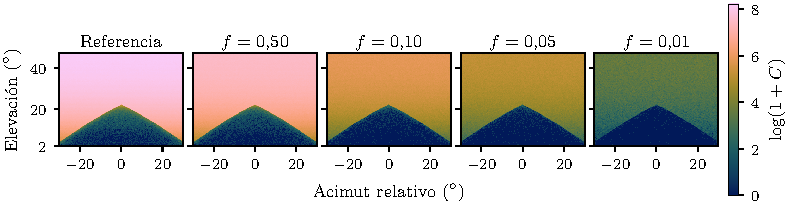
\includegraphics{fig3-4_ejemplo_pares.pdf}
\caption[Ejemplo de un par de baja y alta estadística]{Imágenes de la vista~0 de geo-train-08: referencia ($3{,}44\times10^{8}$ primarios) y primera realización de las entradas obtenidas por adelgazamiento binomial con fracciones 0,50, 0,10, 0,05 y 0,01, en la escala común $\log(1+C)$, donde $C$ es el conteo del píxel. Fuente: elaboración propia a partir del archivo de pares de la campaña de 114 vistas, cuyas huellas de contenido se verificaron antes de generar la figura.}
\label{fig:pares}
\end{figure}

El adelgazamiento binomial depende de la implementación del generador de números aleatorios de la biblioteca numérica, de modo que reconstruir los pares con otra versión puede producir realizaciones distintas; por ello, el procedimiento fija la versión 2.4.4 de NumPy. Además, la huella de un archivo comprimido depende de la versión de la biblioteca de compresión con que se escribió, aunque su contenido sea idéntico. Por esa razón, cada archivo de pares se identificó con dos huellas: la del archivo y la de su contenido, calculada para cada arreglo sobre su tipo de dato, su forma y sus bytes en orden contiguo, de modo que la comparación del contenido no depende de la compresión (sección~\ref{subsec:met-reproduccion}).

\subsection{Partición por geometría y reserva de datos}
\label{subsec:met-particiones}

El conjunto se particionó por geometrías completas: todas las vistas, fracciones y realizaciones de una geometría pertenecen a la misma partición. Si la partición se hubiera hecho por imágenes, las realizaciones de una misma vista, que comparten la referencia, habrían quedado repartidas entre entrenamiento y prueba, con una fuga de información que sobrestimaría el desempeño de los modelos \parencite{kaufman2012}. La asignación siguió el rol fijado para cada geometría en el catálogo (\cref{tab:catalogo}), y se verificó que existieran 114 archivos de pares, seis por geometría, que ninguna geometría apareciera en más de una partición, que la partición de generalización fuera exactamente geo-gen-01 y que las demás tuvieran doce, tres y tres geometrías. La \cref{tab:particion} resume la partición.

\begin{table}[htbp]
\centering
\caption[Partición del conjunto de datos]{Partición del conjunto de datos de la campaña de 114 vistas. Fuente: elaboración propia a partir del inventario del empaquetado del repositorio de referencia.}
\label{tab:particion}
\small
\begin{tabular}{@{}lrlrr@{}}
\toprule
Partición & Geometrías & Identificadores & Pares & Proporción \\
\midrule
Entrenamiento & 12 & geo-train-01 a geo-train-12 & 5\,760 & 63,2\,\% \\
Validación & 3 & geo-val-01 a geo-val-03 & 1\,440 & 15,8\,\% \\
Prueba & 3 & geo-test-01 a geo-test-03 & 1\,440 & 15,8\,\% \\
Generalización & 1 & geo-gen-01 & 480 & 5,3\,\% \\
\midrule
Total & 19 & & 9\,120 & 100,0\,\% \\
\bottomrule
\end{tabular}
\end{table}

Al asignar geometrías completas, las proporciones de la partición quedan determinadas por el número de geometrías de cada rol y no pueden ajustarse de forma continua. Con doce, tres y tres geometrías, la división entre entrenamiento, validación y prueba se aproxima a la proporción 70/15/15 prevista en el plan de trabajo, y la geometría de generalización se reservó adicionalmente fuera de ella. La independencia entre particiones no elimina, sin embargo, que todas compartan las hipótesis del generador y del transporte. En la capa de acceso a los datos empleada por los objetivos siguientes, las particiones de prueba y de generalización se protegieron con una salvaguarda que impide leerlas salvo mediante una autorización explícita, para que no pudieran consultarse de forma inadvertida durante el desarrollo de los modelos.

\subsection{Preprocesamiento, normalización y aumento de datos}
\label{subsec:met-preprocesamiento}

El preprocesamiento no forma parte del producto del OE1: los archivos de pares almacenan conteos crudos, y las transformaciones que se describen a continuación se aplican al cargarlos en los objetivos siguientes, en un único módulo del repositorio del proyecto. Se definieron dos convenciones de entrada, que comparten la escala logarítmica de la referencia de la vista y difieren en el tratamiento de la amplitud. Ambas se presentan en la \cref{eq:preproc}:
\begin{subequations}\label{eq:preproc}
\begin{align}
\kappa &= \log\!\left(1+\max_q C^{\mathrm{ref}}(q)\right), \qquad x^{\mathrm{ref}}=\frac{\log\!\left(1+C^{\mathrm{ref}}\right)}{\kappa}, \label{eq:preproc-escala}\\
x^{\mathrm{low}}_{\mathrm{shared}} &= \frac{\log\!\left(1+C^{\mathrm{low}}\right)}{\kappa}, \label{eq:shared}\\
x^{\mathrm{low}}_{\mathrm{ref\text{-}eq}} &= \frac{\log\!\left(1+C^{\mathrm{low}}/f\right)}{\kappa}, \label{eq:ref-equivalent}
\end{align}
\end{subequations}
donde $\log$ es el logaritmo natural, $\kappa$ es la escala común, $x^{\mathrm{ref}}$ es la referencia normalizada y $x^{\mathrm{low}}$ la entrada normalizada. En la convención compartida (\cref{eq:shared}), la entrada conserva una amplitud del orden de $f$ veces la de la referencia, y la amplificación queda a cargo del modelo. En la convención de referencia equivalente (\cref{eq:ref-equivalent}), los conteos se reescalan por el factor conocido $1/f$ antes del logaritmo; como la transformación es determinista, invertible y disponible en la inferencia, entrada y referencia comparten amplitud y difieren solo en el ruido. La escala $\kappa$ se calcula con la referencia, que no existe cuando solo se dispone de una adquisición corta; para ese caso se previó el estimador operativo $\log\!\left(1+\max_q C^{\mathrm{low}}(q)/f\right)$, que solo requiere la entrada. El uso del máximo de la referencia es, por lo tanto, un contrato de preprocesamiento que debe declararse al interpretar las métricas de imagen.

Se admitieron dos aumentos de datos compatibles con la física de la adquisición. El primero es el reflejo horizontal, aplicado con probabilidad 0,5 sobre el eje de acimut, válido por la simetría de la ventana angular respecto de la dirección de observación; el reflejo vertical se excluyó porque invertiría la dependencia del flujo con la elevación. El segundo es el resubmuestreo, que en cada acceso vuelve a extraer la entrada según la \cref{eq:adelgazamiento}; al aplicar el mismo proceso generativo, constituye un aumento exacto que no modifica la referencia, y se destinó únicamente a la partición de entrenamiento. Ambos aumentos emplean generadores pseudoaleatorios independientes y reproducibles. En el OE2, la implementación corregida sustituyó ambas convenciones por una normalización cuya escala se ajustó solo con la partición de entrenamiento, y no empleó aumentos de datos (sección~\ref{subsec:met-tarea}).

% =============================================================================
\section{Diseño e implementación del modelo de aprendizaje profundo}
\label{sec:met-modelo}

El segundo objetivo específico (OE2) consistió en diseñar e implementar una red generativa antagónica condicional que transformara imágenes muográficas de baja estadística en imágenes próximas a las de alta estadística. El punto de partida fue la implementación desarrollada por los estudiantes en una etapa anterior del proyecto, que ya contenía un generador U-Net, un crítico de parches y un entrenamiento de Wasserstein con penalización de gradiente. Antes de entrenar con el conjunto del OE1, la dirección del proyecto revisó ese código, identificó dos defectos que afectaban la formulación y derivó de él una versión corregida, denominada implementación~v1, que es la que entrenó todos los modelos evaluados en este trabajo. Las arquitecturas se conservaron sin cambios; se modificaron la penalización de gradiente, la normalización de los datos, el contrato de acceso a las particiones y el control del determinismo\footnote{Repositorio \texttt{muografia-documentada}, carpeta del segundo objetivo, rama principal en la revisión \texttt{08cdc0c}; la implementación~v1 conserva la procedencia de cada archivo respecto del código de los estudiantes en el repositorio \texttt{muography-dl-reconstruction}, revisión \texttt{b88fa57}.}. Las secciones siguientes describen la tarea, las dos redes, las funciones de pérdida y la secuencia de entrenamientos y ajustes que condujo a los modelos de la evaluación final.

\subsection{Definición de la tarea y de la entrada condicional}
\label{subsec:met-tarea}

La tarea se planteó como una traducción de imagen a imagen \parencite{isola2017}: a partir de una imagen de conteos de baja estadística de una vista, con fracción $f$, el modelo debe producir una estimación de la imagen de referencia de la misma vista, con la misma malla angular de $256\times256$ píxeles y un solo canal. La salida es una imagen de cuentas equivalentes a la exposición de referencia y no una estimación de densidad ni de opacidad. Se entrenó un modelo por fracción, sin condicionar la red explícitamente por $f$, y, por razones de presupuesto, solo se entrenaron modelos para $f=0{,}05$, de modo que cada vista de entrenamiento aportó veinte pares y cada geometría 120. Con la partición de la \cref{tab:particion}, ello supuso 1\,440 pares de entrenamiento y 360 de validación; las particiones de prueba y de generalización solo se abrieron en la evaluación final (sección~\ref{sec:met-evaluacion}).

La normalización histórica, descrita en la sección~\ref{subsec:met-preprocesamiento}, dividía el logaritmo de los conteos por el de la cuenta máxima de la referencia de cada vista. La revisión de la dirección observó que esa escala depende de la referencia, que no existe cuando solo se dispone de una adquisición corta, y que, en consecuencia, la entrada normalizada cambiaba si cambiaba la referencia. La implementación~v1 la sustituyó por la transformación acotada de la \cref{eq:norm-v1}, cuya escala se ajustó una sola vez con la partición de entrenamiento y se congeló para todas las vistas, fracciones y particiones:
\begin{subequations}\label{eq:norm-v1}
\begin{align}
T(c) &= \frac{\log(1+c)}{s+\log(1+c)}, \qquad s=\log\!\left(1+M_{\mathrm{ent}}\right)=8{,}2393, \label{eq:norm-t}\\
x &= T\!\left(C^{\mathrm{low}}/f\right), \qquad y = T\!\left(C^{\mathrm{ref}}\right), \label{eq:norm-xy}\\
T^{-1}(z) &= \exp\!\left(\frac{s\,z}{1-z}\right)-1, \qquad 0\le z<1, \label{eq:norm-inv}
\end{align}
\end{subequations}
donde $c$ es un conteo no negativo, $M_{\mathrm{ent}}=3\,786$ es la cuenta máxima de las referencias de las doce geometrías de entrenamiento, $x$ es la entrada del modelo, $y$ la referencia normalizada y $T^{-1}$ la transformación inversa, que devuelve cuentas equivalentes. La transformación es monótona, lleva cualquier conteo finito al intervalo $[0,1)$, compatible con la salida sigmoide del generador, y hace que la entrada dependa únicamente de $C^{\mathrm{low}}$, de $f$ y de la escala congelada. Como contrapartida, las métricas calculadas en esta representación no son comparables con las obtenidas con la normalización histórica. La escala quedó registrada en el manifiesto de datos y en cada punto de control de entrenamiento. En la implementación~v1 no se aplicaron aumentos de datos: el reflejo horizontal se desactivó y el resubmuestreo binomial durante el entrenamiento se excluyó, de modo que cada época recorrió los mismos 1\,440 pares.

\subsection{Arquitectura del generador U-Net}
\label{subsec:met-generador}

El generador sigue la arquitectura U-Net \parencite{ronneberger2015}, elegida en la etapa anterior del proyecto mediante ensayos sobre validación. La \cref{fig:arquitecturas} presenta su esquema en el panel~(a). Consta de un codificador de cinco niveles que reduce la resolución de 256 a 16 píxeles y duplica el número de canales hasta 512, y de un decodificador simétrico que recupera la resolución original. Cada nivel aplica un bloque doble formado por dos convoluciones de $3\times3$ con paso unitario, cada una seguida de normalización por instancia y de una activación LeakyReLU con pendiente negativa de 0,2. El submuestreo se realiza por agrupamiento máximo de $2\times2$ y el sobremuestreo mediante convoluciones transpuestas de $2\times2$ con paso 2. En cada nivel del decodificador, el mapa sobremuestreado se concatena con el del mismo nivel del codificador, de modo que la información de alta resolución espacial, en particular la de la silueta del edificio, no tiene que atravesar el cuello de la red. Una convolución final de $1\times1$ seguida de una función sigmoide produce la imagen normalizada $\hat y\in(0,1)$. La red no contiene capas de abandono y tiene 20\,543\,809 parámetros entrenables. La \cref{tab:arquitecturas} detalla los canales, la resolución y los parámetros de cada etapa.

\begin{figure}[htbp]
\centering
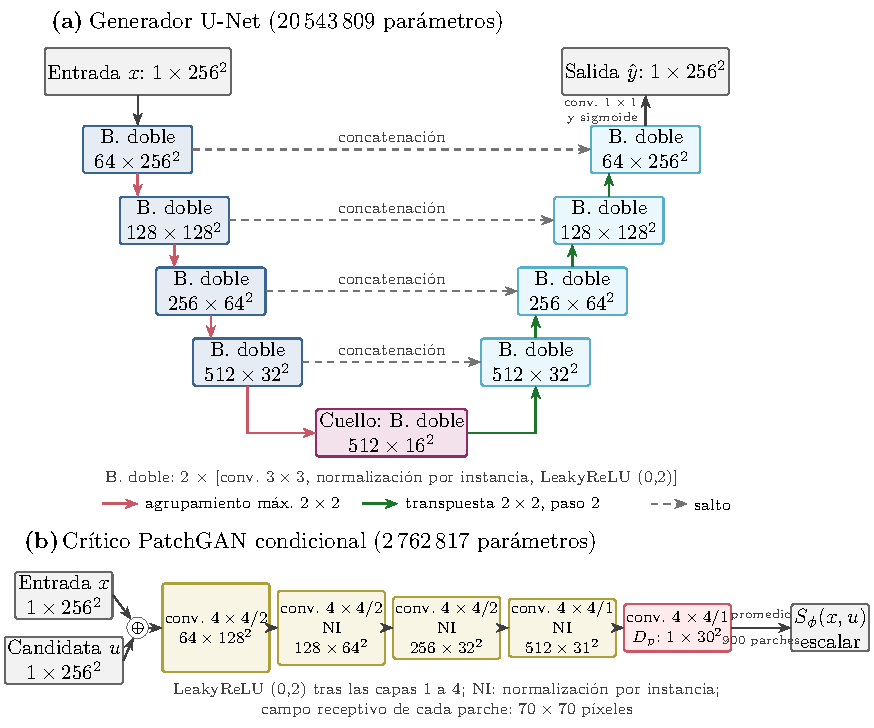
\includegraphics{fig3-5_arquitecturas.pdf}
\caption[Arquitectura del generador U-Net y del crítico PatchGAN]{Arquitectura de las redes del OE2. (a) Generador U-Net de cinco niveles: los bloques indican el número de canales y la resolución de cada nivel; las flechas horizontales discontinuas representan las conexiones de salto por concatenación. (b) Crítico PatchGAN condicional: recibe la entrada de baja estadística concatenada con la imagen candidata y produce un mapa de $30\times30$ puntuaciones, cada una con un campo receptivo de 70 píxeles, que se promedian en una puntuación escalar por muestra. Fuente: elaboración propia a partir de la implementación~v1 del repositorio de referencia.}
\label{fig:arquitecturas}
\end{figure}

\begin{table}[htbp]
\centering
\caption[Etapas del generador y capas del crítico]{Etapas del generador U-Net y capas del crítico PatchGAN de la implementación~v1. B.~doble: dos convoluciones de $3\times3$, cada una con normalización por instancia y LeakyReLU (0,2); NI: normalización por instancia; LReLU: LeakyReLU (0,2); Conv.~$4\times4$/$k$: convolución de $4\times4$ con paso $k$; Agrup.: agrupamiento máximo; Transp.: convolución transpuesta. Fuente: elaboración propia a partir de la implementación~v1 del repositorio de referencia.}
\label{tab:arquitecturas}
\small
\begin{tabular}{@{}llrrr@{}}
\toprule
Etapa & Operación & Canales & Resolución & Parámetros \\
\midrule
\multicolumn{5}{@{}l}{\emph{Generador U-Net}} \\
Codificador 1 & B.~doble & $1\to64$ & 256 & 37\,568 \\
Codificador 2 & Agrup.\ y B.~doble & $64\to128$ & 128 & 221\,440 \\
Codificador 3 & Agrup.\ y B.~doble & $128\to256$ & 64 & 885\,248 \\
Codificador 4 & Agrup.\ y B.~doble & $256\to512$ & 32 & 3\,539\,968 \\
Cuello & Agrup.\ y B.~doble & $512\to512$ & 16 & 4\,719\,616 \\
Decodificador 4 & Transp., salto y B.~doble & $512\to512$ & 32 & 8\,128\,000 \\
Decodificador 3 & Transp., salto y B.~doble & $512\to256$ & 64 & 2\,294\,528 \\
Decodificador 2 & Transp., salto y B.~doble & $256\to128$ & 128 & 573\,824 \\
Decodificador 1 & Transp., salto y B.~doble & $128\to64$ & 256 & 143\,552 \\
Salida & Conv.~$1\times1$ y sigmoide & $64\to1$ & 256 & 65 \\
\midrule
\multicolumn{4}{@{}l}{Total del generador} & 20\,543\,809 \\
\midrule
\multicolumn{5}{@{}l}{\emph{Crítico PatchGAN}} \\
Capa 1 & Conv.~$4\times4$/2, LReLU & $2\to64$ & 128 & 2\,112 \\
Capa 2 & Conv.~$4\times4$/2, NI, LReLU & $64\to128$ & 64 & 131\,072 \\
Capa 3 & Conv.~$4\times4$/2, NI, LReLU & $128\to256$ & 32 & 524\,288 \\
Capa 4 & Conv.~$4\times4$/1, NI, LReLU & $256\to512$ & 31 & 2\,097\,152 \\
Capa 5 & Conv.~$4\times4$/1 & $512\to1$ & 30 & 8\,193 \\
\midrule
\multicolumn{4}{@{}l}{Total del crítico} & 2\,762\,817 \\
\bottomrule
\end{tabular}
\end{table}

\subsection{Arquitectura del crítico PatchGAN}
\label{subsec:met-critico}

El crítico, representado en el panel~(b) de la \cref{fig:arquitecturas}, es un discriminador de parches del tipo PatchGAN \parencite{isola2017}, adaptado a la formulación de Wasserstein. Está condicionado por la entrada: recibe la imagen de baja estadística concatenada en el eje de canales con la imagen candidata, que puede ser la referencia o la salida del generador, y juzga, por tanto, si la candidata es coherente con esa entrada concreta y no solo si parece una imagen muográfica. Consta de cinco convoluciones de $4\times4$, las tres primeras con paso 2 y las dos últimas con paso unitario, con 64, 128, 256, 512 y un canal; las capas intermedias aplican normalización por instancia y todas, salvo la última, activación LeakyReLU con pendiente de 0,2. Como corresponde a un crítico de Wasserstein, la salida no pasa por una sigmoide y no está acotada. El resultado es un mapa de $P=30\times30=900$ puntuaciones $D_p$, cada una asociada a un campo receptivo de $70\times70$ píxeles, equivalente a unos $16{,}4^{\circ}$ de acimut. Ese tamaño se obtiene geométricamente de los núcleos y pasos de las capas; la elección del crítico de 70 píxeles procede de los ensayos de la etapa anterior sobre validación y no de un análisis específico con el conjunto del OE1. El crítico tiene 2\,762\,817 parámetros (\cref{tab:arquitecturas}).

\subsection{Funciones de pérdida y penalización de gradiente}
\label{subsec:met-perdidas}

El entrenamiento antagónico siguió la formulación de Wasserstein con penalización de gradiente (WGAN-GP) \parencite{arjovsky2017,gulrajani2017}, combinada con un término de reconstrucción L1 como en la traducción condicional de imágenes \parencite{mirza2014,isola2017}. Para que la puntuación que se optimiza y la que se regulariza fueran la misma, el mapa del crítico se redujo a una puntuación escalar por muestra mediante su promedio. Las pérdidas del crítico y del generador se presentan en la \cref{eq:wgan}:
\begin{subequations}\label{eq:wgan}
\begin{align}
S_\phi(x,u) &= \frac{1}{P}\sum_{p=1}^{P} D_{\phi,p}(x,u), \label{eq:wgan-score}\\
\mathcal{L}_D &= \frac{1}{B}\sum_{i=1}^{B}\Big[S_\phi\!\left(x_i,\hat y_i\right)-S_\phi\!\left(x_i,y_i\right)\Big]
 + \lambda_{\mathrm{GP}}\,\frac{1}{B}\sum_{i=1}^{B}\Big(\big\|\nabla_{\tilde y}S_\phi(x_i,\tilde y_i)\big\|_2-1\Big)^2, \label{eq:wgan-d}\\
\tilde y_i &= \alpha_i\,y_i+(1-\alpha_i)\,\hat y_i, \qquad \alpha_i\sim\mathcal{U}(0,1), \label{eq:wgan-interp}\\
\mathcal{L}_G &= -\lambda_{\mathrm{adv}}\,\frac{1}{B}\sum_{i=1}^{B}S_\phi\!\left(x_i,\hat y_i\right)+\lambda_{L1}\,\frac{1}{B\,P_y}\sum_{i=1}^{B}\big\|\hat y_i-y_i\big\|_1, \label{eq:wgan-g}
\end{align}
\end{subequations}
donde $D_{\phi,p}$ es la puntuación del parche $p$ del crítico con parámetros $\phi$, $u$ es la imagen candidata, $\hat y_i=G_\theta(x_i)$ es la salida del generador con parámetros $\theta$, $B=4$ es el tamaño del lote, $\tilde y_i$ es una interpolación aleatoria entre la referencia y la salida, $P_y=256\times256$ es el número de píxeles de la imagen, $\lambda_{\mathrm{GP}}=10$ es el peso de la penalización, $\lambda_{L1}=100$ el del término de reconstrucción y $\lambda_{\mathrm{adv}}$ el del término antagónico, igual a 1 en la cGAN. Todas las magnitudes son adimensionales, porque se calculan en el dominio normalizado de la \cref{eq:norm-v1}. La red U-Net de comparación usó el mismo generador con $\lambda_{\mathrm{adv}}=0$, es decir, solo con el término L1, sin crítico.

La revisión del código histórico encontró que la pérdida antagónica usaba el promedio del mapa, mientras que la penalización derivaba su suma. Como el gradiente de la suma es $P$ veces el del promedio, la penalización exigía en realidad que la norma del gradiente de la puntuación promedio fuera $1/P$, y no uno, lo que alteraba el objetivo de la regularización y no solo su escala. La implementación~v1 emplea la misma puntuación $S_\phi$ en la pérdida y en la penalización, como expresa la \cref{eq:wgan-d}, y doce casos analíticos con mapas de $1\times1$, $14\times14$ y $30\times30$ verificaron que la penalización vale cero cuando la norma es uno.

Los ajustes posteriores incorporaron dos términos adicionales, expresados en el espacio de cuentas mediante la inversa de la \cref{eq:norm-v1}. El primero, la pérdida regional de cuentas, penaliza la diferencia entre la cuenta media predicha y la de referencia en las regiones geométricas definidas en la sección~\ref{subsec:met-anomalias}: cielo, roca sin anomalía, borde del cono y anomalías. El segundo, la pérdida espacial de borde, penaliza el error absoluto de cuentas, píxel a píxel, en la franja del borde. Ambos se definen en la \cref{eq:perdidas-cuentas}:
\begin{subequations}\label{eq:perdidas-cuentas}
\begin{align}
\ell_R &= \left|\log\!\left(1+\overline{\hat C}_R\right)-\log\!\left(1+\overline{C^{\mathrm{ref}}}_R\right)\right|, \qquad
\mathcal{L}_{\mathrm{reg}} = \frac{1}{B}\sum_{b=1}^{B}\frac{1}{|\mathcal{F}_b|}\sum_{F\in\mathcal{F}_b}\frac{1}{|F|}\sum_{R\in F}\ell_R, \label{eq:perdida-reg}\\
\mathcal{L}_{\mathrm{borde}} &= \frac{1}{B}\sum_{b=1}^{B}\frac{\sum_{q\in E_b}\left|\hat C_b(q)-C^{\mathrm{ref}}_b(q)\right|}{\sum_{q\in E_b}C^{\mathrm{ref}}_b(q)}, \label{eq:perdida-borde}\\
\mathcal{L}_G^{\mathrm{aj}} &= \mathcal{L}_G+\lambda_{\mathrm{reg}}\,\mathcal{L}_{\mathrm{reg}}+\lambda_{\mathrm{b}}\,\mathcal{L}_{\mathrm{borde}}, \label{eq:perdida-total}
\end{align}
\end{subequations}
donde $\overline{\hat C}_R$ y $\overline{C^{\mathrm{ref}}}_R$ son las cuentas medias predichas y de referencia en la región $R$, $\hat C=T^{-1}(\hat y)$, $\mathcal{F}_b$ es el conjunto de familias de regiones con soporte de al menos veinte píxeles en la imagen $b$, $E_b$ es la región de borde de esa imagen, $\lambda_{\mathrm{reg}}$ es el peso del término regional y $\lambda_{\mathrm{b}}$ el del término de borde. Las cuatro familias pesan lo mismo y, dentro de la familia de anomalías, cada anomalía pesa lo mismo. El término regional se calculó en doble precisión mediante una identidad logarítmica que evita formar exponenciales grandes. Las máscaras intervienen solo durante el entrenamiento: el generador no las recibe y, en la inferencia, procesa únicamente la imagen de baja estadística.

El peso $\lambda_{\mathrm{reg}}=1$ se adoptó como primera hipótesis acotada, sin calibrarlo con validación. El peso del término de borde se fijó antes de su ensayo, con una regla de presupuesto de gradientes evaluada sobre doce lotes de entrenamiento, uno por geometría, con las redes iniciales congeladas y sin consultar la validación. La regla, recogida en la \cref{eq:lambda-borde}, limita la contribución del término de borde al 10\,\% de la norma del gradiente del generador en la mediana de los lotes y al 25\,\% en el peor lote:
\begin{equation}\label{eq:lambda-borde}
r_j=\frac{\left\|\nabla_\theta\mathcal{L}_{\mathrm{borde},j}\right\|_2}{\left\|\nabla_\theta\mathcal{L}^{\mathrm{C0}}_{G,j}\right\|_2}, \qquad
\lambda_{\mathrm{b}}=\frac{1}{1000}\left\lfloor 1000\,\min\!\left(1;\ \frac{0{,}10}{\operatorname{med}_j r_j};\ \frac{0{,}25}{\max_j r_j}\right)\right\rfloor,
\end{equation}
donde $r_j$ es el cociente de normas en el lote $j$ y $\mathcal{L}^{\mathrm{C0}}_{G,j}$ es la pérdida del generador sin término de borde. Con una mediana de 0,1588 y un máximo de 0,2413, la regla dio $\lambda_{\mathrm{b}}=0{,}629$. Se trata de un presupuesto de ingeniería que equilibra los términos, no de una tolerancia física.

\subsection{Entrenamiento, ajuste y selección de modelos}
\label{subsec:met-entrenamiento}

Todos los entrenamientos emplearon el optimizador Adam \parencite{kingma2015} con $\beta_1=0$ y $\beta_2=0{,}9$, valores recomendados para WGAN-GP \parencite{gulrajani2017}, tamaño de lote de 4 y cinco actualizaciones del crítico por cada actualización del generador. En cada iteración, el crítico se entrenó cinco veces con una misma salida del generador desacoplada de su grafo, y después el generador se actualizó con una salida nueva. Cada época recorrió los 1\,440 pares de entrenamiento en 360 lotes, en un orden aleatorio derivado de la semilla del ensayo y del número de época, y terminó con la evaluación completa de los 360 pares de validación. No se usaron precisión mixta ni recorte de gradientes. Para que una ejecución pudiera repetirse e interrumpirse sin alterar su resultado, se activaron los algoritmos deterministas de la biblioteca, se fijaron las semillas de todos los generadores pseudoaleatorios y cada punto de control guardó los pesos, los estados de los optimizadores y los de los generadores aleatorios.

El desarrollo del modelo se organizó como una secuencia de ensayos acotados, en la que cada uno respondió a una pregunta concreta planteada por el resultado del anterior y se diseñó antes de ejecutarse. La \cref{tab:ensayos} resume esa secuencia. El primer ensayo, un piloto al 5\,\%, entrenó desde cero la cGAN y la U-Net con idéntico generador, optimizador, semilla, normalización y presupuesto de épocas, de modo que la única diferencia fuera la componente antagónica; su pregunta era si la implementación corregida se entrenaba de forma estable y si esa componente aportaba alguna mejora. Se usó una tasa de aprendizaje de $10^{-4}$, un máximo de treinta épocas y una parada temprana después de ocho validaciones sin una mejora del SSIM de al menos 0,001; el punto de control seleccionado fue el de mayor SSIM medio en validación. Antes del piloto, una etapa técnica de dos épocas con ocho pares verificó en la GPU que el entrenamiento se reanudara tras una interrupción deliberada sin duplicar épocas y que produjera pérdidas, gradientes y métricas finitas; no se exigió en ella ninguna mejora de calidad.

\begin{table}[htbp]
\centering
\caption[Secuencia de ensayos de desarrollo del OE2]{Secuencia de ensayos de desarrollo del OE2. Todos emplearon $f=0{,}05$ y se decidieron con la partición de validación. Las continuaciones partieron de los puntos de control de la época~5 del piloto, con optimizadores nuevos, tasa de aprendizaje de $10^{-5}$ y cinco épocas adicionales. Fuente: elaboración propia a partir de los diseños y configuraciones del repositorio de referencia.}
\label{tab:ensayos}
\small
\begin{tabularx}{\linewidth}{@{}>{\raggedright\arraybackslash}p{2.3cm}>{\raggedright\arraybackslash}X>{\raggedright\arraybackslash}p{3.6cm}>{\raggedright\arraybackslash}p{2.3cm}@{}}
\toprule
Ensayo & Pregunta y variantes & Punto de partida y semillas & Criterio \\
\midrule
Piloto & ¿Se entrena la implementación corregida y aporta la componente antagónica? U-Net con L1 frente a cGAN & Desde cero; 2026100301 & Decisión descriptiva del protocolo \\
Ajuste de la U-Net & ¿Reduce el término regional el sesgo de cuentas? A: L1; B: L1 $+\ \mathcal{L}_{\mathrm{reg}}$ & U-Net del piloto; 2026100302 & Ocho controles \\
Continuación de la cGAN & Ídem en la cGAN. C0: sin $\mathcal{L}_{\mathrm{reg}}$; C1: con $\mathcal{L}_{\mathrm{reg}}$ & cGAN del piloto; 2026100303 & Ocho controles \\
Repetición R1--R3 & ¿Se mantiene la ventaja de C1 al cambiar la semilla? & cGAN del piloto; 2026100401 a 2026100403 & Ocho controles en las tres parejas \\
Ensayo de borde E1 & ¿Reduce el término espacial el error de borde sin perder lo demás? C0: con $\mathcal{L}_{\mathrm{reg}}$; C1: C0 $+\ 0{,}629\,\mathcal{L}_{\mathrm{borde}}$ & cGAN del piloto; 2026100411 a 2026100413 & Nueve controles en las tres parejas \\
\bottomrule
\end{tabularx}
\end{table}

Los ensayos siguientes ajustaron los modelos del piloto mediante continuaciones: partieron de sus pesos de la época~5, con optimizadores nuevos, una tasa de aprendizaje de $10^{-5}$ y exactamente cinco épocas adicionales, sin parada temprana, conservando siempre la quinta. Cada ensayo comparó dos variantes que solo diferían en un término de la pérdida, con la misma semilla y el mismo orden de muestras, de modo que la diferencia entre ellas pudiera atribuirse a ese término. El ajuste de la U-Net y la continuación de la cGAN añadieron la pérdida regional de la \cref{eq:perdida-reg}; la repetición R1--R3 repitió la segunda con tres semillas nuevas, para comprobar si su resultado dependía de la semilla, y el ensayo de borde E1 tomó como control la variante con pérdida regional y le añadió la pérdida espacial de la \cref{eq:perdida-borde}. Las repeticiones miden la estabilidad condicionada a un mismo punto de partida y no la variabilidad de entrenamientos independientes desde cero.

La decisión de cada ensayo se tomó con reglas fijadas en su diseño. En el ajuste, la continuación y la repetición, la variante con el término nuevo debía cumplir, frente a su control y sin redondeo, ocho controles: un indicador regional $Q$ estrictamente menor, ningún $Q$ por geometría mayor, errores de cielo y de borde no mayores, el mismo soporte de contraste, un error de contraste no mayor y un SSIM y un PSNR no menores. El ensayo de borde añadió un noveno control, que exigía un error espacial de borde estrictamente menor. Si se cumplían todos, el resultado se clasificaba como mejora concordante descriptiva; si $Q$ se reducía pero fallaba algún otro control, como compromiso; y, en otro caso, como ausencia de mejora del indicador principal. En la repetición y en el ensayo de borde, la concordancia exigía que las tres parejas cumplieran todos los controles. Ningún resultado de estos ensayos otorgaba aceptación física.

Durante la continuación de la cGAN se detectó que, en la GPU, un entrenamiento reanudado desde un punto de control no reproducía bit a bit al continuo a partir de la segunda época, aunque sí en procesador. El diagnóstico localizó la primera diferencia en los gradientes del crítico y mostró que los gradientes de la pérdida de Wasserstein y de la penalización eran exactos por separado, mientras que su suma dentro de una misma retropropagación difería en el orden de $4\times10^{-7}$. La corrección, adoptada en todas las continuaciones posteriores y descrita en el algoritmo~\ref{alg:critico}, calcula ambos gradientes por separado, los suma y aplica un único paso del optimizador, sin modificar la pérdida ni introducir tolerancias. Con ella, la reanudación reprodujo exactamente los pesos, los estados de los optimizadores y de los generadores aleatorios, los registros y las predicciones. Como el cambio de controlador de la GPU entre el diagnóstico y la aceptación no permitió aislar su efecto causal, la conclusión se limita al entorno y a la batería de pruebas empleados. El piloto se había entrenado antes de esta corrección, con la retropropagación conjunta.

\begin{algorithm}[htbp]
\caption{Iteración de entrenamiento de la cGAN con gradientes del crítico separados}
\label{alg:critico}
\begin{algorithmic}[1]
\Require lote $\{(x_i,y_i)\}_{i=1}^{B}$; generador $G_\theta$; crítico $D_\phi$; pesos $\lambda_{\mathrm{GP}}$, $\lambda_{\mathrm{adv}}$, $\lambda_{L1}$, $\lambda_{\mathrm{reg}}$, $\lambda_{\mathrm{b}}$; máscaras regionales del lote; número de pasos del crítico $n_D=5$
\Ensure parámetros actualizados $\theta$ y $\phi$
\State $\hat y_i \gets G_\theta(x_i)$ sin propagar gradientes hacia $\theta$ \Comment{salida reutilizada por el crítico}
\For{$n \gets 1$ \textbf{hasta} $n_D$}
  \State extraer $\alpha_i\sim\mathcal{U}(0,1)$ y formar $\tilde y_i$ (\cref{eq:wgan-interp})
  \State $L_W \gets \frac{1}{B}\sum_i\left[S_\phi(x_i,\hat y_i)-S_\phi(x_i,y_i)\right]$; \ $L_P \gets \lambda_{\mathrm{GP}}\,\frac{1}{B}\sum_i\left(\|\nabla_{\tilde y}S_\phi(x_i,\tilde y_i)\|_2-1\right)^2$
  \State $g_W \gets \nabla_\phi L_W$; \ después $g_P \gets \nabla_\phi L_P$ \Comment{dos retropropagaciones separadas}
  \If{alguna pérdida o gradiente no es finito} detener el entrenamiento \EndIf
  \State asignar $g_W+g_P$ como gradiente de $\phi$ y aplicar un paso de Adam
\EndFor
\State congelar $\phi$; \ $\hat y_i \gets G_\theta(x_i)$; \ $\hat C_i \gets T^{-1}(\hat y_i)$
\State calcular $\mathcal{L}_G^{\mathrm{aj}}$ con las \cref{eq:wgan-g,eq:perdida-total} y aplicar un paso de Adam sobre $\theta$
\end{algorithmic}
\end{algorithm}

Cada continuación en GPU fue precedida por una etapa técnica de aceptación, en la que una ejecución continua y otra interrumpida y reanudada debían producir resultados idénticos, y por pruebas en procesador de las pérdidas, del orden de los gradientes y de la conservación de los puntos de control. Los pesos de todas las ejecuciones quedaron identificados por su huella SHA-256 y los ocho que intervinieron en la evaluación final se fijaron en su contrato antes de la inferencia (sección~\ref{subsec:met-protocolo}).

\subsection{Métodos de referencia y estudios de ablación}
\label{subsec:met-comparadores}

Se emplearon dos comparadores. El primero es la entrada sin red, escalada a cuentas equivalentes mediante $C^{\mathrm{low}}/f$ y normalizada con la \cref{eq:norm-xy}; es el resultado que se obtendría sin procesamiento alguno y, por construcción, conserva en esperanza las cuentas de la referencia (\cref{eq:pares-media}), aunque con todo su ruido. El segundo es la U-Net entrenada solo con el término L1, que comparte con la cGAN el generador, la normalización, la semilla, el optimizador y el presupuesto de épocas, y permite atribuir al término antagónico la diferencia entre ambas. En la etapa anterior del proyecto se había empleado también un filtro clásico; como no se reimplementó con la normalización~v1 ni sobre el conjunto del OE1, no formó parte de las comparaciones de este trabajo. Los ensayos de ajuste funcionaron como estudios de ablación de un solo factor: en cada pareja, las dos variantes compartieron el punto de partida, la semilla, el orden de muestras y todos los hiperparámetros, y solo difirieron en la presencia del término regional o del término de borde.

% =============================================================================
\section{Protocolo de evaluación y estimación de la reducción de adquisición}
\label{sec:met-evaluacion}

\subsection{Diseño de la evaluación y criterios de aceptación}
\label{subsec:met-protocolo}

Los ensayos de desarrollo descritos en la sección~\ref{subsec:met-entrenamiento} se decidieron exclusivamente con la partición de validación. Una vez concluidos, la evaluación de los modelos sobre las particiones reservadas se fijó en un protocolo escrito, denominado EF-01, registrado el 4 de octubre de 2026 antes de calcular cualquier métrica de desempeño sobre esas particiones. El protocolo formuló tres preguntas: cuánto recupera la cGAN respecto de la entrada de baja estadística, cómo se compara con la U-Net entrenada con pérdida L1 y qué efecto conservan, fuera de validación, los ajustes de conservación regional y de borde. Su alcance se limitó a la fracción $f=0{,}05$, la única con modelos entrenados, y a la referencia idealizada de alta estadística del OE1; la salida evaluada es una imagen de cuentas equivalentes y no una estimación de densidad.

Se compararon nueve métodos sobre exactamente los mismos pares: la entrada sin red, escalada a cuentas equivalentes mediante $C^{\mathrm{low}}/f$, y ocho redes congeladas, cuyos pesos quedaron identificados por su huella SHA-256 en un contrato ejecutable antes de la inferencia. La \cref{tab:metodos-ef01} presenta esos métodos y su papel en la comparación. Las seis continuaciones del ensayo de borde se incluyeron completas, como análisis secundario, y no como una búsqueda de la mejor semilla; las tres parejas comparten la inicialización de la cGAN original y, por lo tanto, no estiman la variabilidad de entrenamientos independientes desde cero. El protocolo prohibió cambiar de época o de modelo según los resultados reservados y promover automáticamente el mejor valor de una tabla.

\begin{table}[htbp]
\centering
\caption[Métodos comparados en la evaluación final]{Métodos comparados en la evaluación final EF-01 con fracción $f=0{,}05$. Todas las redes se congelaron antes de la inferencia sobre las particiones reservadas. Fuente: elaboración propia a partir del protocolo EF-01 del repositorio de referencia.}
\label{tab:metodos-ef01}
\small
\begin{tabularx}{\linewidth}{@{}>{\raggedright\arraybackslash}p{3.0cm}>{\raggedright\arraybackslash}X>{\raggedright\arraybackslash}p{3.4cm}@{}}
\toprule
Método & Origen & Papel \\
\midrule
Entrada sin red & Conteos de baja estadística escalados por $1/f$ & Comparador sin procesamiento \\
U-Net original & Piloto; generador entrenado solo con pérdida L1; época 5, elegida en validación & Red de referencia \\
cGAN original & Piloto; cWGAN-GP con término L1; época 5, elegida en validación & Modelo principal \\
B1, B2, B3 -- C0 & Cinco épocas adicionales desde la cGAN original con pérdida regional de cuentas; quinta época & Análisis secundario \\
B1, B2, B3 -- C1 & Igual que C0, con el término espacial de borde añadido; quinta época & Análisis secundario \\
\bottomrule
\end{tabularx}
\end{table}

Las particiones de prueba y de generalización se evaluaron por separado. La prueba comprende tres geometrías, dieciocho vistas y 360 imágenes de entrada; la generalización, la geometría geo-gen-01, con seis vistas y 120 imágenes. Las ocho redes produjeron 3\,840 predicciones, que se compararon con las 480 entradas sin red; ninguna de ellas es una simulación nueva, pues todas proceden de los pares del OE1 con fracción 0,05.

Se fijaron de antemano seis comparaciones por partición, doce en total: la cGAN original frente a la entrada, la U-Net frente a la entrada, la cGAN original frente a la U-Net y, dentro de cada pareja B1, B2 y B3, la variante C1 frente a C0. Para cada comparación, geometría y métrica se calculó la diferencia entre el candidato y el comparador, y se registró si el candidato no empeoraba. La clasificación de la comparación sigue la \cref{eq:clasificacion}:
\begin{subequations}\label{eq:clasificacion}
\begin{align}
\delta_{g,m} &= M_{g,m}^{\mathrm{cand}} - M_{g,m}^{\mathrm{comp}}, \qquad
\nu_{g,m} = \begin{cases} 1 & \text{si } \sigma_m\,\delta_{g,m}\ge 0,\\ 0 & \text{en otro caso,}\end{cases} \label{eq:clasificacion-delta}\\
\text{clase} &= \begin{cases}
\text{sin deterioro en las métricas listadas} & \text{si } \nu_{g,m}=1 \ \ \forall\, g,m,\\
\text{compromiso o deterioro} & \text{si } \exists\, g,m:\ \nu_{g,m}=0,
\end{cases} \label{eq:clasificacion-clase}
\end{align}
\end{subequations}
donde $M_{g,m}$ es el valor de la métrica $m$ en la geometría $g$, promediado sobre sus imágenes, y $\sigma_m=+1$ para las métricas en las que un valor mayor es mejor (SSIM y PSNR) y $\sigma_m=-1$ para las de error (el indicador regional, los errores de cielo y de borde y el error de contraste), definidas en las secciones~\ref{subsec:met-calidad} y~\ref{subsec:met-anomalias}. Si alguna métrica no podía calcularse, la comparación se clasificaba como incompleta. La clasificación es descriptiva: la ausencia de deterioro no implica equivalencia ni superioridad estadística.

El plan de trabajo formuló el OE2 en términos de imágenes de calidad comparable a las de alta estadística. Sin embargo, ni el plan ni los protocolos previos fijaron un margen de equivalencia física justificado para las métricas de imagen ni para la conservación de cuentas, y el protocolo EF-01 excluyó expresamente la posibilidad de fijar ese umbral después de conocer los resultados. En consecuencia, la evaluación cuantifica concordancias y limitaciones, y una mejora frente a la entrada o frente a la U-Net no se interpreta, por sí sola, como equivalencia con la referencia.

Antes de iniciar la inferencia se registró una declaración de procedencia de las particiones reservadas. Los ocho modelos no se entrenaron, validaron ni seleccionaron con datos de prueba o de generalización: sus contratos de datos solo admitían archivos de entrenamiento y validación, y el lector de datos rechazaba las demás particiones (sección~\ref{subsec:met-particiones}). No obstante, las mismas cuatro escenas se habían simulado y evaluado en septiembre de 2026 con la versión inicial del conjunto y con modelos de la misma arquitectura, y esos resultados fueron conocidos por los autores y por la dirección. Como no puede descartarse que ese conocimiento influyera en decisiones posteriores, la evaluación EF-01 se presenta como una \emph{evaluación descriptiva sobre datos potencialmente expuestos} y no como una confirmación independiente. Este rótulo se conserva en todos los resultados del capítulo~\ref{chap:resultados}.

Conviene distinguir, por último, tres clases de decisiones. Los compromisos del plan de trabajo fijaron la arquitectura condicional, las particiones y las métricas generales. Las decisiones experimentales de la secuencia de ensayos se tomaron con validación y se describen en la sección~\ref{subsec:met-entrenamiento}. Los análisis posteriores a la apertura de las reservas, que son la corrección numérica de la selección de controles de contraste (sección~\ref{subsec:met-anomalias}) y las curvas descriptivas de exposición (sección~\ref{subsec:met-factor}), se identifican como tales y no modifican los pesos, las predicciones, las particiones ni los criterios del protocolo.

\subsection{Métricas de calidad global de imagen}
\label{subsec:met-calidad}

La calidad global se midió con el índice de similitud estructural (SSIM) y con la relación señal a ruido de pico (PSNR), calculados por imagen en el dominio normalizado de la \cref{eq:norm-v1}, en el que la referencia es $y=T(C^{\mathrm{ref}})$, la entrada sin red es $T(C^{\mathrm{low}}/f)$ y cada red entrega directamente su predicción $\hat y$, todas con rango de intensidad unitario. Ambas métricas se presentan en la \cref{eq:ssim-psnr}:
\begin{subequations}\label{eq:ssim-psnr}
\begin{align}
\mathrm{SSIM}(\hat y, y) &= \frac{1}{|W|}\sum_{w\in W}\frac{\left(2\mu_{\hat y,w}\mu_{y,w}+c_1\right)\left(2\sigma_{\hat y y,w}+c_2\right)}{\left(\mu_{\hat y,w}^{2}+\mu_{y,w}^{2}+c_1\right)\left(\sigma_{\hat y,w}^{2}+\sigma_{y,w}^{2}+c_2\right)}, \qquad c_i=(K_iL)^2, \label{eq:ssim}\\
\mathrm{PSNR}(\hat y, y) &= 10\log_{10}\frac{L^{2}}{\frac{1}{P}\sum_{q=1}^{P}\left(\hat y(q)-y(q)\right)^{2}}, \label{eq:psnr}
\end{align}
\end{subequations}
donde $W$ es el conjunto de ventanas cuadradas de $7\times7$ píxeles con pesos uniformes, $\mu$, $\sigma^2$ y $\sigma_{\hat y y}$ son la media, la varianza y la covarianza locales en cada ventana, $K_1=0{,}01$, $K_2=0{,}03$, $L=1$ es el rango de intensidad y $P=256\times256$ es el número de píxeles \parencite{wang2004}. El PSNR se expresa en decibelios; el SSIM es adimensional y vale uno para imágenes idénticas. Los parámetros se fijaron explícitamente en el código de evaluación para que no dependieran de los valores predeterminados de la biblioteca. Una predicción idéntica a la referencia tendría PSNR infinito; el protocolo previó registrarla como tal, sin confundirla con un valor nulo ni eliminarla, aunque no se presentó ningún caso.

Ambas métricas se resumieron primero por geometría, como media de sus 120 imágenes, y después como media con igual peso de las geometrías de la misma partición. El SSIM y el PSNR miden la semejanza visual y el error cuadrático en la escala logarítmica normalizada, y por ello son sensibles a la reducción del ruido de conteo. No miden, en cambio, si se conservan las cuentas de una región ni el contraste de una anomalía: una imagen suavizada puede obtener valores altos aunque desplace sistemáticamente las cuentas \parencite{hore2010}. Por esa razón se complementaron con los indicadores regionales de la sección siguiente.

\subsection{Regiones de interés y preservación de anomalías}
\label{subsec:met-anomalias}

La conservación física se evaluó en el espacio de cuentas. Cada predicción se transformó de vuelta a cuentas equivalentes con la inversa de la normalización, $\hat C=\exp\!\left(s\hat y/(1-\hat y)\right)-1$, sin recortes ni pseudocuentas, y la entrada sin red se representó por $C^{\mathrm{low}}/f$. Las regiones se derivaron de la geometría de cada escenario y no de las imágenes: para cada píxel se trazó un rayo recto desde la posición nominal del detector, a 1\,000~m del eje del cono y a 1,5~m de altura, hasta una longitud máxima de 3\,000~m, y se calculó su intersección con el cono y con las primitivas de las anomalías. Con esos rayos se definieron cuatro familias de regiones. El \emph{cielo} reúne los rayos que no cortan el cono, erosionados dos píxeles; la \emph{roca sin anomalía}, el interior del cono erosionado dos píxeles y sin las proyecciones de las anomalías, dilatadas otros dos; el \emph{borde}, la franja comprendida entre la dilatación y la erosión de dos píxeles de la silueta del cono, y cada \emph{anomalía}, los rayos que recorren al menos 20~m dentro de ella, erosionados un píxel. El umbral de 20~m es geométrico y no representa una resolución física certificada. Las regiones con menos de veinte píxeles o con cuentas de referencia nulas se registraron como no estimables, igual para todos los métodos, y no se seleccionó ninguna región según el error observado.

Para una región $R$ y una realización $k$ se calcularon el sesgo firmado y el error espacial normalizado de la \cref{eq:regiones}:
\begin{subequations}\label{eq:regiones}
\begin{align}
b_{R,k} &= \frac{\sum_{q\in R}\left(\hat C_k(q)-C^{\mathrm{ref}}(q)\right)}{\sum_{q\in R}C^{\mathrm{ref}}(q)}, \qquad
a_{R,k} = \frac{\sum_{q\in R}\left|\hat C_k(q)-C^{\mathrm{ref}}(q)\right|}{\sum_{q\in R}C^{\mathrm{ref}}(q)}, \label{eq:regiones-ba}\\
Q &= \frac{1}{2}\left(\frac{1}{V}\sum_{v=1}^{V}\left|\bar b_{\mathrm{roca},v}\right| + \frac{1}{V}\sum_{v=1}^{V}\frac{1}{|\mathcal{A}_v|}\sum_{R\in\mathcal{A}_v}\left|\bar b_{R,v}\right|\right), \label{eq:regiones-q}
\end{align}
\end{subequations}
donde $\bar b_{R,v}$ es el sesgo medio de las veinte realizaciones de la vista $v$, $V=6$ es el número de vistas de la geometría y $\mathcal{A}_v$ es el conjunto de regiones de anomalía estimables de la vista $v$. Ambas magnitudes son adimensionales y se expresan en porcentaje de las cuentas de referencia de la región. El indicador regional $Q$ promedia con igual peso el sesgo absoluto de la roca sin anomalía y el de las anomalías, estas últimas promediadas primero dentro de cada vista; resume, por tanto, el desplazamiento sistemático de las cuentas en las regiones físicamente relevantes. No representa un error de densidad ni un porcentaje de error de toda la imagen. Se exigió soporte completo: si una geometría carecía de anomalías o de regiones estimables, $Q$ se informaría como no aplicable, sin sustituirlo por cero. Los errores de cielo y de borde se obtuvieron como la media, sobre las seis vistas, del error espacial $a_{R,k}$ promediado sobre las realizaciones. El error de borde mide la fidelidad píxel a píxel en la transición entre roca y cielo, donde el gradiente de cuentas es máximo.

El contraste de una anomalía se midió frente a controles de roca geométricamente comparables, porque no se dispone de la misma geometría sin anomalía como contrafactual. Para cada píxel del núcleo de una anomalía, excluidos los rayos que atraviesan otra anomalía, se eligieron cinco píxeles de roca sin anomalía de la misma fila de elevación cuya longitud de recorrido dentro del cono difiriera en no más del 5\,\%, escogidos por cercanía de esa longitud. Con esos controles, el contraste y su error se definieron en la \cref{eq:contraste}:
\begin{equation}\label{eq:contraste}
\mathcal{C}_k=\frac{\overline{C}_{\mathrm{obj},k}}{\overline{C}_{\mathrm{ctrl},k}}-1, \qquad
e_{\mathcal{C}}=\frac{1}{K_{\mathrm{v}}}\sum_{k=1}^{K_{\mathrm{v}}}\left|\mathcal{C}_k-\mathcal{C}^{\mathrm{ref}}\right|,
\end{equation}
donde $\overline{C}_{\mathrm{obj},k}$ y $\overline{C}_{\mathrm{ctrl},k}$ son las cuentas medias de los píxeles objetivo y de sus controles en la realización $k$, $\mathcal{C}^{\mathrm{ref}}$ es el mismo contraste calculado sobre la referencia y $K_{\mathrm{v}}$ es el número de realizaciones con control no nulo. El contraste es adimensional y corresponde a la intensidad de conteo, no a la opacidad. Una combinación de anomalía y vista se consideró estimable si reunía al menos veinte píxeles emparejados y una cobertura mínima del 80\,\% de su núcleo; el error medio de cada partición se calculó solo sobre el soporte común, formado por las combinaciones con veinte realizaciones válidas en todos los métodos, cuyo número se informa junto a cada resultado.

Después de abrir las reservas, una reevaluación independiente en otro sistema operativo difirió de la original en cuatro contrastes. El análisis mostró que algunos candidatos a control tenían longitudes prácticamente iguales y que ordenarlos sin tolerancia podía intercambiar el quinto donante por redondeos de la última cifra. La dirección del proyecto estableció entonces la corrección numérica C2, que se resume en el algoritmo~\ref{alg:controles}: se conservan la elegibilidad y los cinco controles por píxel, pero los candidatos cuya diferencia de longitud dista menos de $10^{-8}$~m de la del candidato más cercano se agrupan y se desempatan por columna ascendente, sin encadenar empates. La tolerancia se fijó antes de leer las métricas corregidas, se aplicó por igual a todos los escenarios, anomalías y métodos, y resuelve diferencias próximas a la precisión numérica sin representar una resolución espacial física. Los índices de los controles resultantes se registraron con las huellas de sus máscaras, de modo que una reproducción posterior los reutiliza en lugar de seleccionarlos de nuevo.

\begin{algorithm}[htbp]
\caption{Selección de controles de contraste con tolerancia de empate (corrección C2)}
\label{alg:controles}
\begin{algorithmic}[1]
\Require núcleo de anomalía $\mathcal{T}$; máscara de roca sin anomalía $\mathcal{R}$; longitud de recorrido en el cono $\ell(q)$ de cada píxel; tolerancia relativa $\eta=0{,}05$; número de controles $K_c=5$; tolerancia de empate $\tau=10^{-8}$~m
\Ensure índices de los controles de cada píxel emparejado y su registro con huellas
\For{cada píxel $q\in\mathcal{T}$}
  \State $\mathcal{K}\gets\{r\in\mathcal{R}:\ \text{fila}(r)=\text{fila}(q),\ |\ell(r)-\ell(q)|\le\eta\,\ell(q)\}$
  \State $d(r)\gets|\ell(r)-\ell(q)|$ para cada $r\in\mathcal{K}$; $\mathcal{D}\gets\emptyset$
  \For{cada ancla $d^{*}=\min_{r\in\mathcal{K}} d(r)$, en orden creciente, mientras $|\mathcal{D}|<K_c$ y $\mathcal{K}\neq\emptyset$}
    \State $\mathcal{G}\gets\{r\in\mathcal{K}:\ d(r)-d^{*}\le\tau\}$, sin encadenar empates, ordenado por columna ascendente
    \State añadir a $\mathcal{D}$ los primeros elementos de $\mathcal{G}$ hasta completar $K_c$; \ $\mathcal{K}\gets\mathcal{K}\setminus\mathcal{G}$
  \EndFor
  \If{$|\mathcal{D}|=K_c$} registrar $q$ como emparejado con los controles $\mathcal{D}$ \EndIf
\EndFor
\If{hay al menos 20 píxeles emparejados \textbf{y} cubren al menos el 80\,\% de $\mathcal{T}$}
  \State marcar la combinación como estimable y guardar sus índices y la huella de las máscaras
\Else
  \State marcar la combinación como de geometría insuficiente
\EndIf
\end{algorithmic}
\end{algorithm}

La corrección se verificó con cuatro pruebas específicas, que cubren el orden de empates próximos, la separación entre distancia y elegibilidad, la reproducción con rechazo de índices alterados y el rechazo de soportes modificados, y con 162 comprobaciones de sensibilidad sobre los 54 conjuntos de controles: tolerancias de $10^{-9}$ y $10^{-7}$~m y una perturbación determinista de $\pm10^{-10}$~m en las longitudes, que conservaron exactamente los índices de C2. Estas pruebas acotan la sensibilidad dentro del catálogo, pero no constituyen una garantía universal. La corrección no altera el SSIM, el PSNR ni los indicadores regionales, que no dependen de los controles.

\subsection{Análisis estadístico y tratamiento de la dependencia}
\label{subsec:met-estadistica}

La unidad de inferencia sobre escenarios es la geometría (sección~\ref{subsec:met-enfoque}). Las veinte realizaciones de una vista comparten la referencia y los muones de las entradas son subconjuntos de ella, de modo que no constituyen observaciones independientes; las seis vistas de una geometría comparten, a su vez, el mismo edificio. Con tres geometrías de prueba y una de generalización, el número de unidades independientes es insuficiente para estimar intervalos de confianza o pruebas de hipótesis con interpretación poblacional, y tratarlas como 360 o 120 observaciones independientes habría subestimado la incertidumbre. Por esa razón, el análisis se limitó a la descripción: se informaron las medias por geometría y sus macropromedios con igual peso, se calcularon las diferencias entre métodos para cada geometría y se registró si su signo se repetía en todas ellas. Las comparaciones entre métodos son emparejadas, porque todos se evaluaron sobre las mismas entradas y la misma referencia.

Las particiones de prueba y de generalización se analizaron por separado y nunca se agregaron. La ausencia de diferencias favorables en una comparación no se interpretó como equivalencia, y las diferencias favorables no se interpretaron como superioridad estadística. Las tablas completas por geometría, vista, realización y región se conservaron junto con los macropromedios, para que ninguna conclusión dependa únicamente de un promedio.

\subsection{Estimación del factor de reducción de adquisición}
\label{subsec:met-factor}

La relación entre fracción de conteos y tiempo de adquisición se apoya en el modelo de conteo de la sección~\ref{subsec:met-pares}. Con flujo estable y condiciones de detección iguales, la esperanza del número de muones registrados crece linealmente con la exposición, como expresa la \cref{eq:factor}:
\begin{equation}\label{eq:factor}
\mathrm{E}\!\left[N(t)\right]=\lambda\,t, \qquad
f=\frac{t_{\mathrm{bajo}}}{t_{\mathrm{ref}}}, \qquad
R=\frac{f_{\mathrm{ent}}}{f_{\mathrm{mod}}},
\end{equation}
donde $\lambda$ es la tasa de muones registrados, en muones por unidad de tiempo, $t$ es la exposición, $f$ es la fracción de conteos que conserva una adquisición corta de duración $t_{\mathrm{bajo}}$ frente a la referencia de duración $t_{\mathrm{ref}}$, y $R$ es la razón nominal entre la exposición de una entrada sin red con fracción $f_{\mathrm{ent}}$ y la de la entrada del modelo, con $f_{\mathrm{mod}}=0{,}05$. Con $f=0{,}05$, el factor nominal frente a la referencia completa es $1/f=20$. Como las entradas se construyeron por adelgazamiento de una misma referencia, este factor es una equivalencia idealizada de exposición y no una medición de tiempo de campo; la duración del entrenamiento o de la inferencia tampoco es un tiempo de adquisición.

Determinar un factor alcanzable exige especificar antes qué calidad se considera aceptable. Como ese criterio no se había fijado al cerrar la evaluación del OE2, se realizó únicamente un análisis descriptivo con los datos ya disponibles: se calcularon las mismas métricas de la entrada sin red con las fracciones 0,01, 0,05, 0,10 y 0,50 sobre las particiones reservadas, con la normalización y las regiones del protocolo EF-01, y se compararon con las ocho redes, evaluadas únicamente con $f=0{,}05$. El caso de 0,05 se conservó como control, pues debía reproducir los valores de la entrada en EF-01. Para el contraste se usó el soporte común a las cuatro fracciones y a las ocho redes, porque con la fracción 0,01 algunas realizaciones tienen controles con cero cuentas. Las líneas que unen los cuatro puntos se emplearon solo como guía visual: no se interpoló entre fracciones, no se extrapoló fuera de la rejilla y no se trató la referencia comparada consigo misma como un punto de PSNR infinito. Se distinguieron tres niveles de lectura que no deben confundirse: la reducción nominal de conteos, la equivalencia descriptiva según SSIM y PSNR, y la aceptación física según cuentas y contraste. Este análisis es posterior a la apertura de las reservas y no permite afirmar el desempeño de las redes con otras fracciones de entrada.

\subsection{Generalización, sensibilidad y análisis de fallos}
\label{subsec:met-generalizacion}

La geometría geo-gen-01 se reservó para estimar el comportamiento en un escenario no representado en las particiones de entrenamiento, validación y prueba, y se informó siempre por separado. Al tratarse de una sola geometría, sus resultados describen ese escenario y no una tasa de generalización. La sensibilidad de los resultados se examinó en dos aspectos: la estabilidad numérica de la selección de controles, descrita en la sección~\ref{subsec:met-anomalias}, y la reproducibilidad del cálculo de métricas, que se recalculó de forma independiente en otro equipo a partir de las predicciones conservadas. El análisis de fallos se apoyó en los resultados por geometría y por anomalía, incluidos los cambios de signo del contraste respecto de la referencia, sin seleccionar casos favorables o desfavorables con posterioridad. Todos estos análisis tienen carácter exploratorio, y una buena calidad global de imagen no se equiparó con la detectabilidad física de una anomalía.

% =============================================================================
\section{Entorno computacional, reproducibilidad y trazabilidad}
\label{sec:met-reproducibilidad}

\subsection{Infraestructura y dependencias de software}
\label{subsec:met-entorno}

La simulación del OE1 se ejecutó en el supercomputador SC3 de la Universidad Industrial de Santander, con una cuenta del grupo de investigación. Los ensayos previos y el piloto de seis vistas emplearon la partición \texttt{legacy}, con procesadores Intel Xeon E5645 y 24 hilos por trabajo; la campaña definitiva empleó la partición \texttt{amd}, cuyos nodos cuentan con procesadores AMD EPYC 9554 y 9534, con 64 hilos, 8~GB de memoria y un límite de 15 minutos por trabajo. Antes de la campaña se comprobó la portabilidad de la receta entre ambas particiones: un mismo bloque de $5\times10^{6}$ primarios produjo histogramas idénticos byte a byte con 24 hilos en \texttt{legacy} y con 64 hilos en \texttt{amd}. El entorno de compilación y ejecución se cargó mediante los módulos del clúster para el compilador GCC 14.2.0 y para Geant4 11.4.2, siempre a partir de un entorno limpio, porque las primeras compilaciones enlazaron por error contra la biblioteca estándar del compilador del sistema. EcoMug y la biblioteca de lectura de JSON se incluyeron en el código fuente, de modo que la aplicación puede compilarse sin conexión a internet. La \cref{tab:software} resume las versiones registradas.

Cada componente cumplió un papel preciso en el OE1. Geant4 realizó el transporte de los muones a través del edificio (sección~\ref{subsec:met-transporte}); EcoMug aportó el espectro de momento y la razón de carga por medio de las tablas del generador (sección~\ref{subsec:met-fuente}); y Python implementó el motor analítico, la construcción de las tablas, las validaciones, la publicación y la fusión de los bloques, la evaluación de la calidad, la exportación de las imágenes y la construcción de los pares, con apoyo de las bibliotecas NumPy y SciPy \parencite{harris2020}. El repositorio conserva, además, una receta de contenedor que declara una versión anterior de Geant4; esa receta no se empleó en la campaña y no se ha validado como una vía de reproducción exacta.

\begin{table}[htbp]
\centering
\caption[Versiones de software de la simulación del OE1]{Versiones de software registradas para la simulación del OE1. Fuente: elaboración propia a partir de la receta operativa y de los registros de entorno del repositorio de referencia.}
\label{tab:software}
\small
\begin{tabularx}{\linewidth}{@{}lX@{}}
\toprule
Componente & Versión registrada \\
\midrule
Geant4 & 11.4.2, multihilo; lista de física \texttt{FTFP\_BERT} \\
Compilador & GCC 14.2.0; estándar C++17 \\
EcoMug & 2.2, incluido en el código \\
Biblioteca JSON para C++ & 3.11.3, incluida en el código \\
Posproceso en el clúster & Python 3.13.13, NumPy 2.5.2, SciPy 1.18.1 \\
Construcción de los pares & NumPy 2.4.4 (versión fijada) \\
Receta de contenedor & Geant4 11.3.2 declarado; no validada ni empleada \\
\bottomrule
\end{tabularx}
\end{table}

El entrenamiento y la inferencia del OE2 no se ejecutaron en el supercomputador de la universidad, cuyas GPU estaban ocupadas y cuyo espacio de usuario estaba casi agotado durante el período de los ensayos, sino en un servicio de computación en la nube, con GPU NVIDIA L40S de 46~GB: dos en paralelo en el piloto, una en los ajustes de la U-Net y de la cGAN, tres en paralelo en la repetición y en el ensayo de borde, y una en la evaluación final. Python y PyTorch implementaron las redes, el entrenamiento, la inferencia y la evaluación; scikit-image proporcionó el SSIM y el PSNR, y NumPy y SciPy los cálculos regionales \parencite{harris2020}. El plan de trabajo preveía MATLAB entre sus recursos, pero la implementación heredada de la etapa anterior del proyecto estaba escrita en Python con PyTorch, y no se empleó MATLAB en ninguna etapa. En las continuaciones y en la evaluación final se desactivó la aritmética TF32, de modo que todas las operaciones se realizaron en coma flotante de 32 bits; la configuración del piloto no fijó esa opción de forma explícita. Las reevaluaciones independientes, la corrección del contraste y las curvas de exposición se calcularon en procesador, sin GPU. La \cref{tab:software-oe2} resume las versiones registradas.

\begin{table}[htbp]
\centering
\caption[Versiones de software del modelo y de su evaluación]{Versiones de software y equipos registrados para el entrenamiento y la evaluación del modelo (OE2) y para los análisis posteriores. Fuente: elaboración propia a partir de los registros de entorno del repositorio de referencia.}
\label{tab:software-oe2}
\small
\begin{tabularx}{\linewidth}{@{}lX@{}}
\toprule
Componente & Versión registrada \\
\midrule
Lenguaje y aprendizaje profundo & Python 3.12.3; PyTorch 2.6.0 con CUDA 11.8 y cuDNN 9.1.0 \\
Bibliotecas numéricas & NumPy 2.3.5 (2.4.4 en el piloto); SciPy 1.18.1 \\
Métricas de imagen & scikit-image 0.26.0 \\
Equipo de entrenamiento e inferencia & GPU NVIDIA L40S de 46~GB en un servicio de computación en la nube \\
Reevaluación, corrección C2 y curvas & Python 3.12.14; PyTorch 2.6.0 en procesador; NumPy 2.3.5; scikit-image 0.26.0 \\
\bottomrule
\end{tabularx}
\end{table}

\subsection{Identificación y conservación de datos y modelos}
\label{subsec:met-artefactos}

Cada producto del OE1 quedó identificado por dos elementos complementarios: la semilla que lo generó y una huella criptográfica de su contenido. La huella SHA-256 \parencite{nist2015} identifica de forma unívoca el contenido de un archivo, pues cualquier cambio de un solo byte la altera; por ello se registró en cada etapa: la de la receta y el manifiesto antes del envío, la de los archivos de cada bloque en su recibo de publicación, la de los histogramas fusionados y sus metadatos en el inventario de la fusión, la de cada imagen exportada en el inventario de la exportación y la de cada archivo de pares, junto con las huellas de contenido de sus arreglos, en el inventario del empaquetado. Una fecha, en cambio, solo data el momento en que se fijó un producto: una reconstrucción podría conservarla y producir, aun así, archivos distintos. Por esa razón, la identidad del conjunto se estableció con las huellas y no con fechas. La \cref{tab:semillas} reúne las semillas de la cadena de simulación.

\begin{table}[htbp]
\centering
\caption[Semillas de la cadena de simulación del OE1]{Semillas registradas en la cadena de simulación del OE1. Fuente: elaboración propia a partir del repositorio de referencia.}
\label{tab:semillas}
\small
\begin{tabularx}{\linewidth}{@{}>{\raggedright\arraybackslash}p{6.2cm}>{\raggedright\arraybackslash}X@{}}
\toprule
Uso & Semilla o derivación \\
\midrule
Catálogo de escenarios & 20260805, con un generador independiente derivado por geometría \\
Muestra de EcoMug & 20260805 \\
Validación del muestreador y pruebas físicas del motor analítico & 20260805; la prueba de exactitud de tablas usa 123 \\
Diagnóstico de geo-train-06 y control geométrico & 20260929; la simulación de control T4 usa 2026092900 \\
Ensayo piloto de la corrección & 2026092801, 2026092802 y 2026092803 \\
Campaña definitiva & \cref{eq:semilla-campana}; 1\,026 semillas únicas, distintas de las del piloto de seis vistas \\
Adelgazamiento binomial & semilla maestra 20260805, con derivación por geometría, vista, fracción y realización \\
\bottomrule
\end{tabularx}
\end{table}

El repositorio de referencia conserva el código, las configuraciones, la receta, el manifiesto, los registros del gestor de trabajos, los 114 histogramas fusionados con sus metadatos y las 114 imágenes exportadas, todos con sus inventarios de huellas. Los archivos de pares, que ocupan cerca de 547~MB, se distribuyeron en una copia compartida acompañada de un documento con las versiones, los commits y las huellas empleadas; los 1\,026 bloques publicados, que ocupan unos 734~MB, se conservan en el supercomputador con su inventario de huellas registrado en el repositorio.

En el OE2 se aplicó el mismo principio. Cada configuración de entrenamiento registró su semilla, la partición de entrenamiento, la de selección, la prohibición de acceder a las particiones reservadas, la escala de normalización y la huella del punto de partida, y cada punto de control quedó identificado por su huella SHA-256; las semillas de los ensayos se indican en la \cref{tab:ensayos}. El contrato de la evaluación final fijó las huellas de los ocho pesos, de los archivos de datos de las cuatro geometrías reservadas y del código de evaluación, y el evaluador se negó a ejecutarse si alguna no coincidía. Las 3\,840 predicciones, que forman 32 matrices de $120\times256\times256$ valores en coma flotante y ocupan 1\,006\,637\,056 bytes, se acompañaron de recibos con sus huellas. La corrección C2 guardó, además, los índices exactos de los controles de contraste con las huellas de sus máscaras. Una huella identifica el contenido, pero no data el momento en que se fijó; por ello, la anterioridad del protocolo y de la declaración de procedencia respecto de la inferencia se sustenta en el orden de los registros del repositorio y no en un sello temporal certificado. El repositorio de referencia conserva las configuraciones, los registros, las métricas y las huellas; los pesos y las predicciones, por su tamaño, se distribuyeron en copias compartidas cuyo acceso público se verificó descargando archivos y contrastando sus huellas.

\subsection{Verificación del software y procedimiento de reproducción}
\label{subsec:met-reproduccion}

La integridad del conjunto se verificó con herramientas que no ejecutan simulaciones ni modifican los datos, acompañadas de pruebas automáticas con datos sintéticos que cubren, entre otros, manifiestos y máscaras alterados, semillas y ejecutables incorrectos y campañas incompletas. La reproducción se entendió en dos niveles. El primero, la reproducción desde los datos originales, repite los cálculos a partir de las entradas primarias y compara los productos resultantes con los registrados. En ese nivel se repitió la evaluación de calidad desde los histogramas fusionados, con el plan, la receta y las máscaras congelados; se comprobó que las imágenes exportadas conservaran exactamente los conteos y las coordenadas de los histogramas, y se regeneraron los 9\,120 pares desde las 114 imágenes, de forma independiente, en una segunda máquina de los estudiantes y en la revisión de la dirección, en ambos casos con NumPy 2.4.4. Como las huellas de los archivos comprimidos dependen de la biblioteca de compresión, la regeneración se contrastó con las huellas de contenido de los 342 arreglos de los pares. Por último, la copia de distribución se recuperó desde su enlace con una cuenta distinta de la propietaria y se contrastó, archivo por archivo, con los inventarios del repositorio.

Para el transporte, en cambio, no se dispuso de una segunda ejecución independiente de la campaña: la verificación se apoyó en los registros del gestor de trabajos, en los recibos de cada bloque y en la prueba de portabilidad entre particiones descrita en la sección~\ref{subsec:met-entorno}. Durante el proyecto, una reconstrucción de los pares del conjunto inicial con otra versión de la biblioteca numérica había producido realizaciones binomiales distintas, lo que llevó a fijar la versión empleada y a verificar las huellas al terminar cada construcción.

El segundo nivel, el recálculo a partir de valores almacenados, reconstruye tablas y totales desde los metadatos y registros, como la suma de los primarios transportados y registrados de la campaña o las horas de cómputo asignadas. Ese recálculo comprueba la coherencia interna de los registros, pero no constituye una reproducción, porque no vuelve a generar los datos.

En el OE2, la reproducción desde los datos originales se verificó en varios puntos. En el entrenamiento, la aceptación técnica de cada continuación exigió que una ejecución interrumpida y reanudada reprodujera exactamente a la continua (sección~\ref{subsec:met-entrenamiento}). En la inferencia de los ajustes, la repetición y el ensayo de borde, los pesos se volvieron a aplicar en procesador sobre las imágenes de validación, y las diferencias por píxel frente a las predicciones de la GPU no superaron $10^{-5}$. En la evaluación final, la revisión de la dirección recalculó, desde las 3\,840 predicciones y las 480 entradas, las métricas de todas las imágenes, que coincidieron exactamente, y las regionales, con diferencias máximas de $4{,}44\times10^{-16}$; además, volvió a inferir con los pesos originales cuatro imágenes de una geometría de prueba por cada red, con una diferencia máxima de $4{,}85\times10^{-6}$, comprobación que es una muestra y no una repetición completa de la inferencia. Una segunda evaluación completa con el registro de controles de la corrección C2 reprodujo su informe byte a byte, y en el análisis de exposición el caso de 0,05 reprodujo los valores de la entrada de la evaluación final con una tolerancia de $10^{-12}$. No se repitió, en cambio, ningún entrenamiento completo de forma independiente: la reproducibilidad del entrenamiento se apoya en la recuperación exacta y en las huellas, no en una segunda ejecución. Las tablas del capítulo~\ref{chap:resultados} se recalcularon a partir de las métricas almacenadas, lo que comprueba su coherencia con los registros pero no constituye una reproducción.

\subsection{Trazabilidad de decisiones y limitaciones metodológicas}
\label{subsec:met-decisiones}

La generación del conjunto se realizó en tres pasadas. La primera empleó el motor analítico para validar el diseño de extremo a extremo con un costo computacional mínimo. La segunda sustituyó el motor analítico por el transporte con Geant4, con el mismo catálogo y el mismo formato de datos, y dio lugar al conjunto inicial. La tercera incorporó las decisiones derivadas de su revisión técnica: la construcción corregida de las anomalías, la malla angular de intervalos iguales, la inyección junto a la roca con margen angular de 5°, el umbral de registro de 3~GeV, el número fijo de primarios por vista y los criterios de calidad registrados antes del envío. La dirección del proyecto adoptó el alcance idealizado del producto y acordó con los estudiantes, antes de la campaña, el presupuesto de $3{,}44\times10^{8}$ primarios por vista, la meta descriptiva de roca y el tratamiento de las vistas que no la alcanzaran. Se optó por una campaña nueva, en lugar de completar las vistas del piloto, para no alterar sus recibos ni la definición de la evaluación confirmatoria.

La metodología del OE1 tiene limitaciones que conviene declarar antes de presentar sus resultados. En la geometría, los escenarios son conos idealizados sin topografía circundante; no se dispuso de un control independiente para los volúmenes que sobresalen del edificio en geo-gen-01 y geo-test-03, y los casos que combinan recorte y sustracción múltiple no se ensayaron por separado. En la fuente, el modelo híbrido y su extensión fuera de la ventana son hipótesis del conjunto y no un flujo calibrado. En el transporte, solo se siguieron muones primarios, sin partículas secundarias, respuesta instrumental ni fondo experimental, y el plano de conteo es una superficie computacional que no equivale a un detector físico de 1,2~m, cuya equivalencia no se demostró. En la normalización, la exposición es una escala convencional y la referencia ideal de cielo no incluye pérdidas en el aire, desintegración, dispersión ni migración angular. En el muestreo, las veinte realizaciones de una vista comparten su referencia y la referencia conserva su propio ruido, y las máscaras de roca ignoran las anomalías. Por último, en la procedencia, la versión de EcoMug empleada en la muestra no quedó fijada a una revisión exacta y algunos insumos históricos de las primeras etapas no se conservaron. Las consecuencias observadas de estas limitaciones se analizan en el capítulo~\ref{chap:resultados}.

El desarrollo del modelo se apartó del plan de trabajo en varios aspectos que conviene declarar. Se entrenaron modelos para una sola fracción, $f=0{,}05$, en lugar de la campaña de entrenamientos con las cuatro fracciones que se había previsto; las arquitecturas se heredaron de la etapa anterior y no se volvieron a seleccionar con el conjunto del OE1; el filtro clásico de esa etapa no se incluyó en las comparaciones, y el cómputo se realizó en la nube y no en el supercomputador. La dirección del proyecto revisó el código heredado y estableció las correcciones de la implementación~v1, aprobó la secuencia de ensayos, autorizó la evaluación final, estableció la corrección numérica del contraste y dio por cerrada la parte experimental del OE2 sin pedir más entrenamientos. Ninguna de esas decisiones fijó un margen de equivalencia física, de modo que la expresión del plan sobre una calidad comparable a la de alta estadística no pudo convertirse en un criterio de aceptación.

Las limitaciones del OE1 se transmiten al modelo: las referencias son idealizadas y conservan su propio ruido, las realizaciones de una vista comparten la referencia y las imágenes no equivalen a las de un detector físico. A ellas se suman las propias del OE2. Las continuaciones comparten la inicialización y no estiman la variabilidad desde cero; las particiones reservadas contienen tres geometrías de prueba y una de generalización, ya evaluadas en una etapa anterior; el indicador regional resume sesgos de cuentas en regiones geométricas y no errores de densidad, y la normalización depende de una escala ajustada con la partición de entrenamiento. En el OE3, el factor nominal de reducción es una equivalencia idealizada derivada del adelgazamiento binomial y no un tiempo de campo medido. Las consecuencias observadas de estas limitaciones se analizan en el capítulo~\ref{chap:resultados}.
